\documentclass[12pt,a4paper,catalan]{article}
\usepackage[utf8]{inputenc}
\usepackage{graphicx} % for images
\usepackage{booktabs} % for tables
\usepackage{fancyhdr} % for header and footers
\usepackage{titlesec}
\usepackage{hyperref} % for links 
\usepackage{minted}
\usepackage{amsmath} % for math annotations
\usepackage{todonotes}
\usepackage{enumitem}
\usepackage{amsfonts}
\usepackage{subcaption}
\usepackage[catalan]{babel}
\usepackage{cite}
%\usepackage{caption}
%\usepackage{siunitx}


%Definició de noms:
\newcommand{\titleTFG}{Ciència de les dades aplicada a resultats acadèmics}
\newcommand{\myname}{Xavier Moreno Liceras}



\setlength{\parindent}{0pt}

%Definició de colors:
\definecolor{bgcode}{rgb}{0.93, 0.93, 0.93}

%\setcounter{secnumdepth}{4}
%\setcounter{tocdepth}{4}
\titleformat{\paragraph}
{\normalfont\normalsize\bfseries}{\theparagraph}{1em}{}
\titlespacing*{\paragraph}
{0pt}{3.25ex plus 1ex minus .2ex}{1.5ex plus .2ex}

% define letters
\makeatletter
\def\iddots{\mathinner{\mkern1mu\raise\p@
\vbox{\kern7\p@\hbox{.}}\mkern2mu
\raise4\p@\hbox{.}\mkern2mu\raise7\p@\hbox{.}\mkern1mu}}
\makeatother

\pagestyle{fancy}
\fancyhf{}
\rhead{\titleTFG}
\cfoot{\thepage}
 
\hypersetup{
    unicode=true,          % non-Latin characters in Acrobat’s bookmarks
    pdftitle={\titleTFG},    % title
    pdfsubject={TFG},
    pdfauthor={\myname},     % author
    pdfproducer={\LaTeX},   % producer
    pdfcreator={\myname},   % creator of the document
    pdfkeywords={tutor} {innovació docent} {predicció} {pla d'acció tutorial}, % list of keywords
    colorlinks=true,       % false: boxed links; true: colored links
    linkcolor=blue,          % color of internal links (change box color with linkbordercolor)
    citecolor=blue,        % color of links to bibliography
    urlcolor=blue           % color of external links
}

\begin{document}

\bibstyle{plain}
\thispagestyle{empty}

\begin{titlepage}
\begin{center}
\begin{figure}[h]
\begin{center}

\includegraphics[width=6cm]{img/ub.png}
\end{center}
\end{figure}

\textbf{\LARGE Treball final de grau} \\
\vspace*{.5cm}
\textbf{\LARGE GRAU D'ENGINYERIA INFORMÀTICA } \\
\vspace*{.5cm}
\textbf{\LARGE Facultat de Matemàtiques \\ Universitat de Barcelona} \\
\vspace*{1.5cm}
\rule{\textwidth}{0.1mm}\\
\begin{Huge}
\textbf{\titleTFG} \\
\end{Huge}
\rule{\textwidth}{0.1mm}\\

\vspace{1cm}

\begin{flushright}
\textbf{\LARGE Autor: \myname}

\vspace*{2cm}

\renewcommand{\arraystretch}{1.5}
\begin{tabular}{ll}
\textbf{\Large Directora:} & \textbf{\Large Laura Igual } \\
\textbf{\Large Realitzat a:} & \textbf{\Large  Departament   } \\
 & \textbf{\Large Matemàtica Aplicada y Anàlisis} \\
\\
\textbf{\Large Barcelona,} & \textbf{\Large \today }
\end{tabular}

\end{flushright}

\end{center}
\end{titlepage}

\pagenumbering{roman}

\todo{Ha de ser redactat en primer persona del plural del present}
\todo{Revisió de les faltes d'ortografia}


\section*{\textit{Abstract}}

\textit{Aquest treball està dins del marc d'un projecte d'innovació docent, en el que es proposa una eina de suport per al tutor d'estudis, la qual permeti ajudar al tutor a conèixer millor el perfil de cada alumne que tutoritza. Per poder arribar a fer aquest sistema intel·ligent per al tutor d'estudis, abans s'ha de fer un anàlisi estadístic sobre els resultats acadèmics de la Facultat de Matemàtiques. L'anàlisi es basa en l'exploració de perfils d'estudiants i en la predicció de notes. Dins de l'anàlisi de perfils d'estudiants es mira la tassa d'abandonament per cada perfil i la relació que té cadascun respecte els perfils del curs anterior. Pel que fa a la predicció es construeix una taula de ranking de dificultats d'assignatures per a un alumne.}

\section*{\textit{Resum}}
\textit{Aquest treball està dins del marc d'un projecte d'innovació docent, en el que es proposa una eina de suport per al tutor d'estudis, la qual permeti ajudar al tutor a conèixer millor el perfil de cada alumne que tutoritza. Per poder arribar a fer aquest sistema intel·ligent per al tutor d'estudis, abans s'ha de fer un anàlisi estadístic sobre els resultats acadèmics de la Facultat de Matemàtiques. L'anàlisi es basa en l'exploració de perfils d'estudiants i en la predicció de notes. Dins de l'anàlisi de perfils d'estudiants es mira la tassa d'abandonament per cada perfil i la relació que té cadascun respecte els perfils del curs anterior. Pel que fa a la predicció es construeix una taula de ranking de dificultats d'assignatures per a un alumne.}


\section*{\textit{Resumen}}
\textit{Este trabajo está dentro del marco de un proyecto de innovación docente, en el que se propone una herramienta de soporte para el tutor de estudios, la cual permita ayudar al tutor a conocer mejor el perfil de cada alumno que tutoriza. Para poder llegar a hacer este sistema inteligente para el tutor de estudios, antes hay que hacer un análisi estadístico sobre los resultados académicos de la Facultad de Matemáticas. El análisi se basa en la exploración de perfiles de estudiantes i en la predicción de cualificaciones. Dentro del análisi de perfiles de estudiantes se mira la tasa de abandono para cada perfil i la relación que tiene cada uno respecto los perfiles del curso anterior. Respecto a la predicción se construye una tabla de ranking de dificultad de assignaturas para un alumno.}


\newpage 

\addto\captionsenglish{
  \renewcommand{\contentsname}%
    {Índex}%
}


{\hypersetup{linkcolor=black}
	\thispagestyle{empty}
	\tableofcontents
	\thispagestyle{empty}
}

\newpage

\pagenumbering{arabic} 
\setcounter{page}{1}


\section{Introducció}
Un dels components bàsics de l'activitat docent és l'acció tutorial, la qual té com a finalitat guiar i aconsellar a l'estudiant durant la seva etapa d'estudis. Ajuda a l'estudiant a millorar el seu rendiment, a la seva orientació professional, i el més important, ajuda a prendre decissions que afavoreixin els seus estudis i la seva satisfacció. Per un altre banda tenim el pla d'acció tutorial (PAT) que tracta d'un document amb un conjunt ordenat d'accions sistemàtiques previament planificades. Una de les coses que impulsa el PAT és l'assignació d'un tutor d'estudis a un grup d'estudiants. Un tutor d'estudis té com a finalitat, entre altres, acompanyar a l'alumnat durant el seu transcurs estudiantil des de l'inici del grau, fins al final, donant consell cara al món professional.
\\
\\
Ens hem trobat amb el problema que un tutor d'estudis al tutoritzar a un grup d'alumnes, no és capaç de contemplar detingudament cadascun d'aquests. Els pot guiar de forma genèrica, així seguint el pla d'acció tutorial. S'ha pogut observar al llarg dels anys, per exemple, que alumnes amb qualificacions moderades a primer i segon del grau d'Enginyeria Informàtica tenen problemes per afrontar certes assignatures de tercer. Això s'ha pogut observar al llarg dels anys, però i si estem evitant altres problemes o fets que no s'han pogut obervar fins ara? És això el que volem explorar i fer conclusions que no s'hagin pogut arribar. Arran de tot això, s'ha fet una petició al Vicerectorat de Política Docent per dur a terme un projecte que facilités el treball al tutor d'estudis. D'aquí neix el projecte com un projecte d'innovació docent, amb el títol de: \textit{Sistema intel·ligent de suport per al tutor d'estudis}.
\\
\\
La finalitat del projecte d'innovació docent és la creació d'una eina que el tutor pugui consultar i li ajudi a prendre decissions cara a les seves tutories. Aquesta eina ha de permetre al tutor visualitzar la trajectoria d'un alumne, fer recomanacions específiques per cadascun d'ells, entre altres. Un dels recursos principals d'aquest projecte són les dades, ja que són la que ens permetran arribar a conclusions i poder construïr l'eina per al tutor d'estudis. Les dades han sigut obtingudes a través del Vicerectorat de Política Docent.
\\
\\
Aquest treball forma part del projecte d'innovació docent, i ens centrem en l'estudi estadístic dels resultats acadèmics de la Facultat de Matemàtiques de la UB. L'objectiu és montar una base per poder montar en la següent fase del projecte el sistema per al tutor d'estudis. En aquest treball ens hem centrat en l'exploració dels perfils d'estudiants dels primers cursos de cadascun dels graus impartits en la Facultat de Matemàtiques. També s'ha treballat en un sistema de predicció de notes d'un alumne cara a la seva próxima matriculació. A més s'ha desenvolupat un ranking de dificultat de notes no matriculades d'un alumne a partir d'un predictor de notes. L'objectiu general d'aquest treball és obtenir coneixement a partir de les dades, i és per això que hem convertit aquest projecte en un projecte de ciència de les dades.


\newpage


\section{Descripció del problema}
\subsection{Projecte d'innovació docent}
Aquest treball de fi de grau, ve arran d'un projecte d'innovació docent \cite{pid} que va nèixer del Departament de Matemàtica Aplicada i Anàlisi (MAIA) i Departament de Metòdes de Investigació i Diagnòstic en Educació (MIDE). El participants del projecte són:
\begin{itemize}[leftmargin=.5in]
	\item Dra. Laura Igual Muñoz (MAIA)
	\item Dr. Santiago Seguí Mesquida (MAIA)
	\item Dr. Eloi Puertas Prats (MAIA)
	\item Dr. Oriol Pujol (MAIA)
	\item Dr. Jordi Vitrià Marca (MAIA)
	\item Dra. Petia Radeva (MAIA)
	\item Dr. Luís Garrido Ostermann (MAIA)
	\item Dra. Maria  del Pilar Folgueiras Bertomeu (MIDE)
\end{itemize}

Com ja s'ha dit, la finalitat del projecte d'innovació docent és el desenvolupament d'un sistema intel·ligent de suport al tutor d'estudis, i per dur-lo a terme el projecte s'ha dividit en 5 fases.

\subparagraph{Fase 1}
Adquisició, ordenació, centralització i anonimització de les dades curriculars disponibles dels alumnes. La fase inicial on es deixen les dades preparades per poder treballar amb elles.

\subparagraph{Fase 2}
Anàlisi de les dades mitjançant tècniques de ciències de les dades. Fer un anàlisi estadístic de les dades que tenim i aplicar ciència de les dades per explorar la informació amagada darrere de les dades.

\subparagraph{Fase 3}
Anàlisi de les dades mitjançant tècniques d’aprenentatge automàtic. A partir de les dades aplicar algoritmes de predicció de dades per poder predir les notes d'un alumne en base a les seves notes i la de la resta.

\subparagraph{Fase 4}
Desenvolupament del sistema intel·ligent. En aquesta fase es busca el desenvolupament de la eina de suport per al tutor d'estudis.

\subparagraph{Fase 5}
Avaluació. S'avalua el sistema per tal de fer proves, i buscar mancances i errors del propi sistema.
\\
\\
Aquest treball forma part de la fase 1, 2 i 3. Les fases 4 i 5 són l'altre part del projecte, i no s'en parlarà en aquest treball.

\subsection{Ciència de les dades}
La ciència de les dades és el conjunt d'etapes per tal d'arribar a un resultat, en forma de coneixement, a partir d'un conjunt de dades. Aquesta aplica un conjunt de tècniques de diferents àreas, ara com matemàtiques, estadística, teoria de la informació o tecnologia de l'extracció d'informació.
\\
\\
Un projecte de ciència de les dades es separa en diverses etapes:
\begin{enumerate}
	\item \textbf{Plantejament de preguntes} Què és el que volem explorar? Té sentit el que ens estem plantejant?
	\item \textbf{Adquisició de les dades} Com és la font d'obtenció de les dades? (Base de dades, \textit{Web Scraping}, fitxer .csv)
	\item \textbf{Descripció} Aquesta fase abasta tres processos
	\begin{enumerate}
		\item \textbf{Neteja de dades} Com hem de netejar i separar les dades? (mostres atípiques, filtració, redució de dimensions, normalització, extracció de característiques)
		\item \textbf{Agregació} Com hem de recolectar i resumir les dades? (promig, desviació estàndard, box plots)
		\item \textbf{Enriquiment} Com podem afegir més informació a les nostres dades? (Cerca a altres fonts de dades adicionals)
	\end{enumerate}
	\item \textbf{Descobriment} Podem segmentar les nostres dades per trobar grups naturals i disgregats? (Clusterització, visualització)
	\item \textbf{Anàlisis} Com hem de modelar les nostres dades? (Com estan de relacionades cada variable?, Com podem determinar quines són les variables importants?)
	\item \textbf{Predicció} A partir de les dades que tenim, que podem predir del futur? (Regresions, classificadors, recomanadors)
	\item \textbf{Evaluació} Com de segur estem dels nostres resultats? (Proves estadístiques, rendiment del model)
\end{enumerate}

\subsection{Etapes del projecte}

\subsubsection{Plantejament de preguntes}
La primera etapa és el plantejament de les preguntes que voliem resoldre. A partir de la plataforma trello (explicada en la secció d'eines), entre els participants del projecte vam plantejar preguntes, les quals entre tots decidiem amb quines preguntes ens quedariem i respondriem. Moltes de les preguntes no podíem saber si les podíem respondre fins que ens arribessin les dades, ja que depeniem totalment de la informació que contenien aquestes.

\subsubsection{Adquisició}
L'adquisició de les dades va ser a partir del Vicerectorat de Política Docent. Aquest ens va proporcionar les dades a través d'una fulla de càlcul. Tot i que les dades vinguessin anonimitzades i tractades pel departament corresponent, vam haver de fer una neteja de dades.

\subsubsection{Neteja de dades}
En aquesta etapa hem hagut de netejar les dades per tal de poder treballar amb elles. Aquestes van ser les netejes que es van fer:

\subparagraph{Canvi de format}
Com ja s'ha explicat anteriorment les dades van arribar en un full de càlcul, on en cada fulla havia una taula amb diferent informació. Per poder manipular-les millor des de Python, es va separar cada fulla en un fitxer amb format \textit{csv}, de tal manera que va quedar un fitxer \textit{csv} per taula. En la próxima secció s'explica amb detall les dades obtingudes.

\subparagraph{Canvi de nom de les columnes}
Per tal de poder creuar les diferents taules, els noms de les columnes havien de ser el mateix.

\subparagraph{Enriquiment de les dades}
A partir d'una font externa hem pogut adquirir el curs i semestre que es cursa cada assignatura, per tant el que fem és creuar aquestes dades amb les dades que tenim de cada assignatura per tal de tenir més informació per assignatura.

\subparagraph{Unió de graus}
L'any 2009 el grau en Enginyeria Informàtica de la UB tenia com a codi \textit{G1041}, però a partir de l'any 2010 el codi va passar a ser \textit{G1077}. Les assignatures eren les mateixes, tot i que tenien codis diferents també. Vam procedir a fer la unió dels \textit{G1041} amb \textit{G1077}, per tal de no perdre informació rellevant, ni considerar-la per separat.

\subparagraph{Eliminació del curs 2014, segon semestre}
Explorant les dades em vaig adonar que alumnes que s'havien matriculat l'any 2014, però encara no havien acabat de cursar l'assignatura, en aquesta els hi apareix un 0. Això fa que dintre de les notes dels alumnes hi hagin dades incoherents, per aquesta raó es va decidir eliminar totes les notes del segon semestre i de l'any 2014. El percentatge d'eliminació de dades és d'un 10.91\% del total de notes que tenim.

\subparagraph{Normalitació de les notes}
Per tal d'evitar els canvis de mitja i variança en cada assignatura cursada per any, ja sigui per un canvi de professor, canvi de pla docent, diferents promocions, \ldots es va decidir normalitzar les notes per any i per assignatura aplicant una normalització d'unitat tipificada \cite{normtipificada} en la qual s'aplica per cada dada la següent fórmula:
$$ z = \frac{x - \mu}{\sigma}, $$

on $\mu$ és el promig per any i per assignatura, i $\sigma$ és la desviació estàndard per any i per assignatura. Amb això aconseguim mitja 0 i desviació estàndard 1.

\subsubsection{Clusterització}
Aquesta etapa era necessaria per poder respondre a una des les preguntes plantejades, i és: \textit{Hi ha diferents perfils d'alumnes?}. Per tal de  respondre a aquesta pregunta s'han aplicat mètodes de clusterització a partir de les notes dels alumnes diferenciats per cursos.

\subsubsection{Predicció}
La predicció, com s'ha explicat abans, és la predicció del futur a partir de les dades disponibles. En aquest cas hem volgut predir les notes que pot arribar a treure un alumne en base a les notes que ha tret en cursos anteriors.

\subsubsection{Evaluació}
Un cop construida la predicció, hem d'avaluar quant de bona és. S'ha d'evaluar de forma quantitativa (mitjançant mètriques) i qualitativament (amb la mostra de casos).

\newpage

\subsection{Explicació de les dades obtingudes} 
En aquest apartat s'explicarà la informació més rellevant que podem trobar en les nostres dades. Recordem que les dades ens havien arrivat en una fulla de càlcul, i aquesta l'hem separat per diversos fitxers amb format .csv.
\\
\\
Les dades que hem pogut adquirir són molt enriquidores, tenen la informació necesaria per fer un estudi ampli tant per als estudiants com per a l'estudi d'assignatures. A més les dades venen anonimitzades, a priori no podem obtenir la informació d'un alumne que coneguem. Les dades les tenim separades en diferents fitxers, els quals estan relacionats entre si mitjantçant identificadors, com ara un identificador d'alumne o el codi d'una assignatura. Els fitxers són els següents:

\subparagraph{Informació general de l'estudiant}
Aquest fitxer conté per cada fila informació sobre un alumne en termes de matriculació: l'any d'inici de carrera, grau que realitza, la via amb la qual va accedir a la carrera, la nota d'accés a la Universitat, entre altres.

\subparagraph{Informació d'assignatures}
Aquí podem trobar la informació de cada assignatura que existeix en els graus d'Enginyeria Informàtica i matemàtiques. Per cada fila tenim la següent informació: l'identificador de l'assignatura, el nom de l'assignatura, els crèdits ECTS corresponents a aquesta i el grau a la que pertanyen. A més a més, vam obtenir mitjantçant una altre font d'informació, per cada assignatura de quin curs i semestre es tractava. Aquesta dada la vam creuar amb l'anterior per ampliar la informació per assignatura.

\subparagraph{Qualificacions per alumne i per assignatura}
Per últim i més important, el fitxer que conté les qualificacions de tots els alumnes per assignatura, és a dir, per cada fila tenim: l'identificador de l'alumne que realitze l'assignatura, l'identificador de l'assignatura realitzada, la qualificació d'aquella assignatura, l'ensenyament del qual es tracta, l'any en el que es va realitzar l'assignatura i el tipus d'apunt (ordinaria, reconeixement o convalidada).

\newpage

\subsection{Preguntes plantejades}
\paragraph{Hi ha diferents perfils d'alumnes?}
A partir de la distribució de les notes de cada alumne per cada assignatura que ha fet, podem determinar que hi ha diferents perfils d'estudiants? Això és el que ens estem preguntant. S'han agafat tots els alumnes que hagin cursat totes les assignatures de primer i després les de segon, tant al grau d'Enginyeria Informàtica com al grau de matemàtiques. La experiència ens diu que hi han alumnes bons en programació i dolents en les assignatures de matemàtiques a primer del grau d'Enginyeria Informàtica. Però per a la resta de cursos, quins perfil podem trobar? Ara que tenim les dades això ho podem saber, convertirem les dades en coneixement.

\paragraph{Quina és la tassa d'abandonament per cada tipus de perfil?}
A partir dels perfils que han sigut determinats en la pregunta anterior, quin és el percentatge d'abandonament per cadascun d'aquests. Volem saber si és cert que els alumnes que van a parar al perfil d'alumnes que ho suspenen tot són els que solen abandonar la carrera. Fins ara això és el que podem saber a partir de l'experiència, però es pot demostrar amb dades i corroborar-ho.

\paragraph{Amb quin perfil de provinença encaixa cadascun d'aquests perfils?}
Al llarg dels anys s'ha pogut notar que els alumnes que solen treure bones notes a primer d'Enginyeria Informàtica, acaben treien bones notes a segon la gran majoria. Ara bé, això és cert? Per això ens plantegem aquesta pregunta, a partir de perfils d'origen, volem saber amb quin perfil de destí solen anar. En aquest cas hem fet els següents creuaments per cada grau:

\begin{table}[h]
\centering
\begin{tabular}{@{}cc@{}}
\toprule
{\bf Origen}               & {\bf Destí}                \\ \midrule
Via d'accés                & Perfil d'alumnes de primer \\
Perfil d'alumnes de primer & Perfil d'alumnes de segon  \\ \bottomrule
\end{tabular}
\end{table}

Els perfils d'alumnes de primer i segon són els perfils determinats a la primera pregunta, i els perfils de via d'accés que hem seleccionat han sigut els següents:
\begin{enumerate}
	\item Batxillerat (Batx)
	\item Salt d'Universitat (Uni)
\end{enumerate}

Hem obviat els alumnes provinents de cicle o ja diplomants, per la seva baixa presència. Les vies d'accés només les comprovem amb els alumnes que hagin cursat totes les assignatures de primer, sense convalidar, el que fa que no apareguin una gran quantitat d'alumnes de cicle, ja que la majoria d'aquests tenen alguna assignatura convalidada de primer. I pel que fa als alumnes ja diplomats, no hi han masses en totes les dades presents.

\paragraph{Predicció de notes i ranking de dificultat d'assignatures}
A partir de les notes que ha tret un alumne en el seu passat, podem predir quines assignatures li aniran bé i malament en el futur? Bé, això és el que ens plantejem en aquesta última pregunta, volem recomanar a un alumne en quines assignatures no li aniran gaire bé per a que així pugui reforçar més el temari que es donarà en aquella assignatura. Recordem que la finalitat del projecte d'innovació docent és que aquesta eina sigui un suport per al tutor, és a dir, la predicció no ens dirà el que ha de fer un alumne, aquesta decisió es delega al tutor que a partir de l'eina decidirà que fer.
\newpage

\section{Planificació}
\subsection{Tasques}
Les tasques d'aquest projecte són semblants a les etapaes d'un projecte de ciència de les dades. Les tasques són:
\begin{itemize}[leftmargin=.5in]
	\item Formació
	\item Plantejament de preguntes
	\item Neteja de dades
	\item Clusterització
	\item Predicció
	\item Evaluació
	\item Documentació
\end{itemize}

Les úniques etapes noves que trobem són: la de formació, és la etapa dedicada l'aprenentatge autònom de les eines utilitzades; la de documentació, és el període de temps per tal de desenvolupar aquesta memòria.

\newpage

\subsection{Diagrama de Gantt}
S'ha construït dos diagrames de Gantt, un a partir de la planificació inicial i l'altre amb la planificació real per tal de veure les diferències.

\begin{figure}[h]
\begin{center}
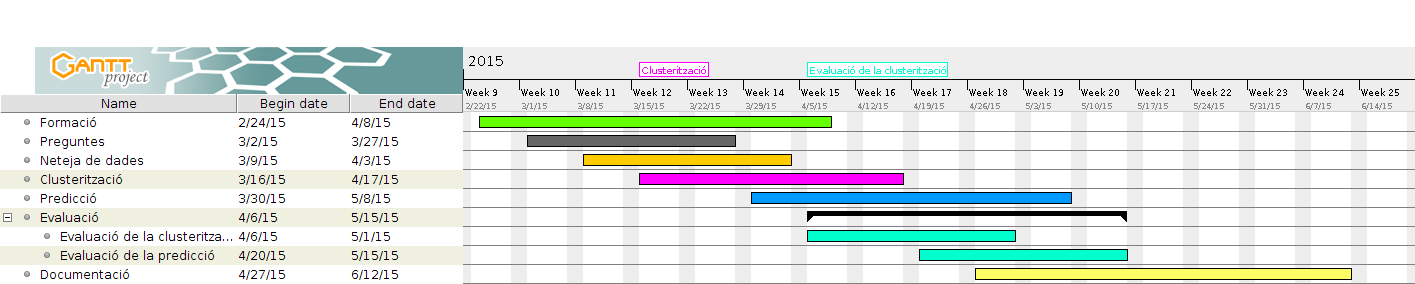
\includegraphics[width=\linewidth]{img/initialplanification.png}
\caption{Planificació inicial}
\end{center}
\end{figure}


\begin{figure}[h]
\begin{center}
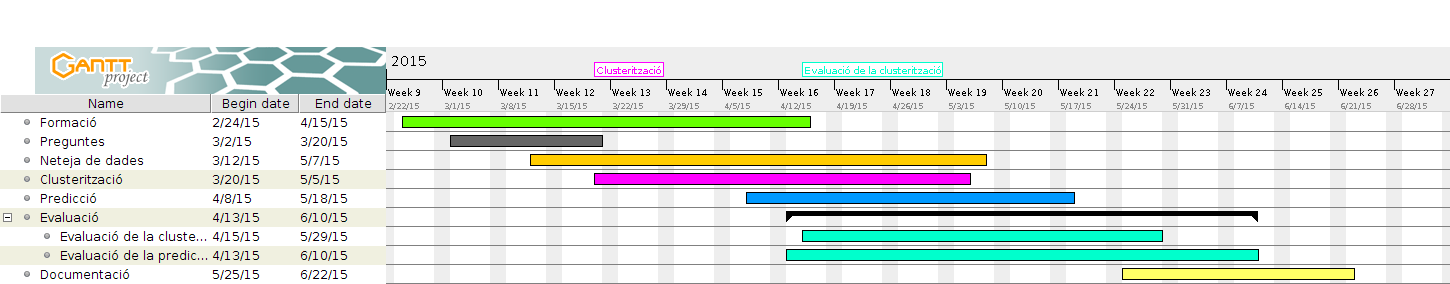
\includegraphics[width=\linewidth]{img/realplanification.png}
\caption{Planificació real}
\end{center}
\end{figure}

El Treball de fi de Grau equival a 18 crèdits ECTS, si cada crèdit equival a 25 hores, llavors tenim:

$$18\,cr\grave{e}dits \cdot \frac{25\,hores}{1\,cr\grave{e}dits} = 450\,hores$$

Per tant totes les tasques s'han de dividir en 450 hores, les hores dedicades han sigut les següents:

\begin{table}[h]
\centering

\begin{tabular}{@{}llllllll@{}}
      & \rotatebox{90}{Formació} & \rotatebox{90}{Preguntes} & \rotatebox{90}{Neteja de dades} & \rotatebox{90}{Clusterització} & \rotatebox{90}{Predicció} & \rotatebox{90}{Evaluació} & \rotatebox{90}{Documentació} \\ \midrule
Hores & 25       & 25        & 50              & 75             & 75        & 125       & 50           \\ \bottomrule
\end{tabular}
\caption{Hores de dedicació per cada tasca}
\end{table}

\newpage

\subsection{Evaluació económica}



\begin{table}[h]
\centering

\begin{tabular}{@{}llll@{}}
\toprule
                & Hores & Preu per hora (Euro) & Preu total (Euro) \\ \midrule
Formació        & 25    & 0                 & 0              \\
Plantejament de preguntes       & 25    & 10                & 250            \\
Neteja de dades & 50    & 20                & 1000           \\
Clusterització  & 75    & 25                & 1875           \\
Predicció       & 75    & 25                & 1875           \\
Evaluació       & 125   & 25                & 3125           \\
Documentació    & 75    & 0                 & 0              \\ \midrule
TOTAL           & 450   &                   & 8125           \\ \bottomrule
\end{tabular}
\caption{Taula d'evaluació económica}
\end{table}

El projecte sortiria per 8125 euros, en els quals s'inclou en la etapa de Evaluació, una documentació dels resultats obtinguts i les conclusions d'aquests.

\newpage

\section{Desenvolupament del projecte}
\subsection{Eines}
\subsubsection{Eines de suport}
Aquestes són les eines de suport que ens han ajudat al llarg del treball per tal de fer més còmode la seva organització tant personal com per equip.

\paragraph{GitHub}
GitHub \cite{github} és una plataforma online per desenvolupar projectes software de forma col·laborativa. Aquesta plataforma utilitza un control de versions anomenat Git. La finalitat de GitHub és l'emmagatzenament massiu de projectes amb codi font obert. Per això hem optat per la utilització de GitHub, ja que que volem que el nostre codi el pugui veure tothom i que qualsevol que el necessiti per fer la seva investigació, el pugui utilitzar.

\paragraph{Bitbucket}
Bitbucket \cite{bitbucket} és una plataforma semblant a GitHub, però amb el servei d'un altre control de versions com Mercurial a més de Git. Bitbucket té l'advantatge de permetre crear repositoris privats de forma gratuïta. Aquesta plataforma va bé per a l'inici d'un projecte on es fan molts canvis en el codi, ja que pots tenir el codi en privat, i un cop el codi ja agafa forma es pot migrar a GitHub. Això és el que hem fet nosaltres en el projecte, començar amb Bitbucket i després passar-nos a GitHub amb el codi font obert.

\paragraph{Trello}
Per últim com eina de suport, hem fet servir Trello \cite{trello}, una plataforma online que permet una comunicació més clara entre els membres d'un projecte. Amb Trello pots crear projectes i cada projecte conté un conjunt de llistes que s'omplen de tasques. Hem fet servir Trello per comunicar-nos amb la tutora i tenir present una planificació per tal d'organitzar-nos millor.

\newpage
\subsubsection{Eines de programació}
En aquesta secció trobarem amb el llenguatge de programació, i conjunt de llibreries, que hem treballat.

\paragraph{Python}
Python \cite{python} és un llenguatge d'alt nivell interpretat. Remarquen molt la fàcil lectura del seus codis, per això té una sintaxis molt semblant a un pseudocodi. Python és un llenguatge de codi obert i desenvolupat per \textit{Python Software Foundation}, una organització sense ànim de lucre. Vam escollir Python per dues raons: per ser un llenguatge de scripting i per la seves llibreries relacionades amb el tractament de dades (com \hyperlink{pandas}{Pandas}, \hyperlink{numpy}{NumPy} o \hyperlink{sklearn}{Scikit-learn}).


\hypertarget{pandas}{
	\paragraph{Pandas}
}
Pandas \cite{pandas} és una biblioteca informàtica escrita en Python per a la manipulació i anàlisi de dades. Especialment va bé per al tractament de taules alhora de fer consultes, o per a l'agrupació i agrecació d'informació.

\hypertarget{numpy}{
	\paragraph{NumPy}
}
Numpy \cite{numpy} és una biblioteca informàtica de Python per operar amb vectors i matrius d'una forma més extensa a la que et permet el mateix llenguatge Python, la qual conté tot un conjunt de funcions matemàtiques d'alt nivell per treballar amb aquests vectors i matrius.

\hypertarget{sklearn}{
	\paragraph{Scikit-learn}
}
Scikit-learn \cite{sklearn} (o sklearn) és una biblioteca informàtica orientada a l'aprenentatge automàtic per a Python. Té suport per classificadors, regressors i clusterització. Per aquest projecte hem fet servir clustering i regressors. En la secció de \hyperlink{tecniquesutilitzades}{Tècniques utilitzades} es detalla cada tècnica utilitzada d'aquesta biblioteca informàtica.

\paragraph{Bokeh}
Bokeh \cite{bokeh} és una biblioteca informàtica per a la visualització interactiva de dades dirigida als navegadors per a la seva presentació a través d'HTML i JavaScript. Bokeh té el suport per a gràfiques específiques com diagrames de barra, box plots o time series, però a banda d'aquests gràfics pots dibuixar sobre un gràfic amb elements bàsics com cercles, línies, rectangles, entre altres.

\paragraph{Seaborn}
Per últim tenim Seaborn \cite{seaborn} que també és una biblioteca informàtica per a visualitazció de dades com Bokeh, amb gràfiques específiques per a la visualització de resultats estadístics. A més té una part dedicada a les paletes de colors i la qual permet escollir un conjunt de colors afavorits per mostrar les dades.

\begin{figure}[h]
\begin{minted}
[
framesep=5mm,
baselinestretch=1.2,
bgcolor=bgcode,
fontsize=\footnotesize
]
{python}
%matplotlib inline
import seaborn as sbn
palette = sbn.color_palette("hls", 5)
sbn.palplot(palette)
\end{minted}
\begin{center}

\includegraphics[width=8cm]{img/palplot_seaborn.png}
\end{center}
\caption{Elecció d'una paleta de 5 colors}
\end{figure}


\subsubsection{Eines d'edició}
\paragraph{IPython notebook}
Ipython notebook \cite{ipythonnotebook} és un editor per a l'entorn de Python. La filosofia \textit{notebook} s'emprea per tenir un codi molt més llegible i a més tenir explicacions d'allò que es programa, ja que es pot barrejar codi, la sortida del codi, markdown, HTML, entre altres. Hem optat per escollit aquest entorn d'edició ja que en un projecte de ciència de les dades s'han de veure resutats constants i poder-los comentar.

\paragraph{Texmaker}
Texmaker \cite{texmaker} és una eina d'edició de \LaTeX, la qual permet poder generar informes, documents, llibres d'una forma més programàtica. A partir d'un etiquetatge estipulat es poden generar documents amb un estil predefinit com el d'aquesta memòria.

\newpage
\hypertarget{tecniquesutilitzades}{
	\subsection{Tècniques utilitzades}
}
\subsubsection{Clusterització (Agrupacions)}
La clusterització és molt important en el món de les dades, permet reconèixer diferents grups de ítems de les nostres dades, en el nostre cas d'alumnes. Per això, abans de veure els resultats i experiments explorats, cal entendre les diferències entre les diferents tècniques de clusterització. En aquest projecte hem fet servir dues tècniques, on l'objectiu d'elles és el mateix, desframentar les dades i trobar diferents grups d'alumnes. Aquestes dues tècniquies són K-means i MeanShift, ambdues implementades en la biblioteca informàtica de Scikit-learn.

\paragraph{\textit{K-means}}
\textit{K-means} \cite{k-means} probablement és un dels algoritmes d'agrupació més conegut. Partint de $n$ elements, divideix aquests $n$ elements en $k$ grups (argument obligatòri de l'algoritme) on cada element pertany al grup més proper a la mitjana. L'algoritme de \textit{K-means} està descrit per la següent fórmula:
\\
\\
Tenint un conjunt d'elements $(x_1, x_2, \ldots, x_n)$ on cada elements és un vector $d$ dimensional, \textit{K-means} construeix una partició dels elements en $k$ grups, on $k \leq n$ quedant $S = \{S_1, S_2, \ldots, S_k\}$. Amb la finalitat de minimitzar la suma dels quadrats dintre de cada grup:

$$ \underset{S} {arg\,min} \sum_{i=1}^{k} \sum_{x_j \in S_i} \left\| x_j - \mu_i \right\|^2 $$

on $\mu_i$ és el centroide dels punts del conjunt $S_i$, és a dir, el punt mig.
\\
\\
Com es veu en la fòrmula, aquest algoritme depén d'una $k$, per determinar agrupacions, per tant \textit{K-means} ha de rebre com paràmetre d'entrada quants grups busquem. També podem pensar que depén del centroide $\mu_i$, però no es necessari, ja que aquest convergeix si s'apliquen $x$ iteracions sobre la fòrmula.

\newpage

\paragraph{\textit{Mean Shift}}
\textit{Mean Shift} \cite{mean-shift} és l'altre tècnica d'agrupació o clusterització que utilitzo en aquest projecte. L'objectiu d'aquesta tècnica és el mateix que \textit{K-means}, però el seu algoritme funciona de forma diferent, considerant l'espai de característiques com una funció de densitat de probabilitat.
\\
\\
Aquest algoritme no necessita com a entrada el número de clusters que busquem, com \textit{K-means}. Té altres paràmetres d'entrada, però són opcionals. En aquesta imatge podem veure la diferència entre \textit{K-means} i \textit{Mean Shift}.

\begin{figure}[h]
\centering
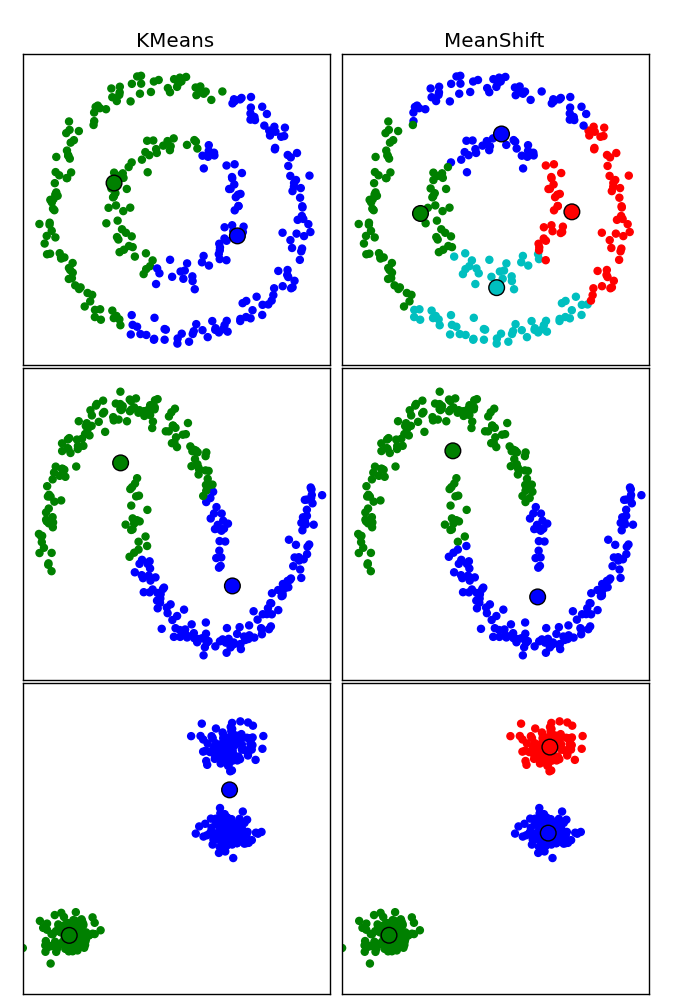
\includegraphics[width=.4\linewidth]{img/kmeansVsMeanshift.png}
\caption{Comparació de K-means amb Mean Shift \cite{comp-meanshift-kmeans}}
\end{figure}

Com es veu en la figura d'adalt, en el tercer gràfic de cada tècnica, tenim que amb \textit{MeanShift}, com no hem de dir el número de divisions que volem, ell mateix ens diu que hi han tres grups. Però amb \textit{K-means} si possem dos clusters, per exemple, estariem unificant dos clusters en un.

\newpage

\paragraph{Mètriques utilitzades}
Existeixen dos indicadors d'avaluació dels resultats de l'anàlisis:
\begin{enumerate}
	\item \textbf{Supervisat} Utilitza les agrupacions reals per comparar-les amb les agrupacions donades per l'algoritme de clusterització.
	\item \textbf{No supervisat} És tot lo contrari, mesura la qualitat del propi model, basant-se en les característiques d'aquest.
\end{enumerate}

En el nostre cas, el que volem és explorar i averiguar quins perfils d'estudiants hi han, per tant hem d'utilitzar mètriques no supervisades, ja que no tenim una referència per comparar. La única mètrica no supervisada que utilitzem és la \textit{Silhouette}.

\subparagraph{\textit{Silhouette}}
Silhouette \cite{silhouette} és una mesura no supervisada, que valora la integrat de cada node dintre d'un cluster. Per cada punt (o observació) calculem la \textit{silhouette} amb la següent fórmula:

$$ s(i) = \frac{b(i) - a(i)}{\max\{a(i),b(i)\}} $$

on:
\begin{itemize}[leftmargin=.5in]
	\item [$i$] és el punt del qual volem calcular la \textit{silhouette}.
	\item [$a(i)$] és la distància mitja als demés punts dintre del cluster de $i$.
	\item [$b(i)$] és la distància mitja als punts que no estan dintre del cluster de $i$.
\end{itemize}

Un cop tenim la \textit{silhouette} calculada per cada observació, per tenir la \textit{silhouette} del cluster, fem la mitja de totes elles.

$$ \mathrm{silhouette_g} = \frac{1}{n} \sum_{j=1}^n silhouette_i $$

\newpage

\subsubsection{Predicció}
La etapa de predicció és important en un projecte de data science, ja que ens permet predir el futur d'una forma estadística en base a les observacions que tenim. Però igual que la clusterització, hi han diverses tècniques, aquí explicaré quines tècniques hem utilitzat per aquest projecte.
\\
\\
Un predictor és un algoritme que pasat un conjunt de dades d'entrenament, és capaç de poder predir dades del futur. En el nostre cas, per exemple entrenem als predictors amb les notes de primer i segon de carrera. Llavors si li pasem un alumne amb les notes de primer, el predictor ens podrà predir quines seran les seves notes de segon basant-se en les dades que li hem passat per entrenar.

\paragraph{Recomanador}
Una de les tècniques per predir dades són els recomanadors. En aquest apartat explicaré com funciona el recomanador que he montat possant-nos en context del nostre projecte. Tenint en compte les notes d'un conjunt d'alumnes, el recomanador és capaç de predir de forma estadística les notes d'un alumne en base a la resta dels altres.
\\
\\
Imaginem que tenim una matriu tal que:
$$
C = \bordermatrix{~ &         a_1   &    a_2   &   \cdots    &    a_m  \cr
                  e_1    &  c_{11}  &     ?    &   \cdots    &  c_{1m} \cr
                  e_2    &  c_{21}  &  c_{22}  &   \cdots    &    ?    \cr
                  \vdots &  \vdots  &  \vdots  &   \ddots    &  \vdots \cr
                  e_n    &    ?     &  c_{n2}  &   \cdots    &  c_{nm} \cr
                  }
$$

on:
\begin{itemize}[leftmargin=.5in]
	\item [$e_i$] és un estudiant.
	\item [$a_i$] és una assignatura.
	\item [$c_{ij}$] és la nota d'un estudiant $i$ en una assignatura $j$.
	\item [$?$] són notes no completes, perquè un alumne no ha cursat l'assignatura.
\end{itemize}

La finalitat del nostre recomanador, és omplir les notes que apareixen amb $?$ i possar la nota més adient. Abans d'explicar com funciona, introduiré els diferents tipus de recomanadors que podem tenir:

\subparagraph{Recomanador col·laboratiu bassat en estudiant (RCxE)}
Prediem la nota d'un alumne en base a la semblança de l'alumne amb la resta. És a dir, si un alumne $e_i$ té unes notes semblants a un alumne $e_j$, les assignatures que no ha cursat $e_i$ podrem dir que seran semblants a les notes que ha tret $e_j$ en aquelles assignatures.

\subparagraph{Recomanador col·laboratiu bassat en assignatures (RCxA)}
Ara en comptes de bassar-nos en la semblança entre els estudiants, ens basem en la semblança entre una assignatura amb la resta. És a dir, si una assignatura $a_i$ segueix una distribució semblant a una assignatura $a_j$, llavors podem dir que un alumne $e_i$ treurà una nota semblant en ambdues assignatures.

\subparagraph{Recomanador híbrid}
Per últim tenim la barreja dels dos recomanadors esmentats, aplicant un pes d'importancia a cadascun. Aquest recomanador no s'ha fet servir en aquest projecte, però es podria fer servir si es pogués apendre quin pes assignar a cada tipus de recomanador.
\\
\\
Començaré explicant el recomanador col·laboratiu bassat en l'estudiant, el qual agafaré com a base per explicar el bassat en assignatures. Imaginem que tenim una matriu semblant a la d'abans:
\\
$$
C = \bordermatrix{~      &   a_1   & \cdots  &           a_q            & \cdots  &   a_m  \cr
                  e_1    &  c_{11} & \cdots  & \textbf{c}_{\textbf{1q}} & \cdots  &    ?   \cr
                  \vdots &  \vdots & \ddots  &     \textbf{\vdots}      & \iddots & \vdots \cr
                  e_p    &    ?    & \cdots  &       \textbf{?}         & \cdots  & c_{pm} \cr
                  \vdots &  \vdots & \iddots &       \textbf{\vdots}    & \ddots  & \vdots \cr
                  e_n    &  c_{n1} & \cdots  & \textbf{c}_{\textbf{nq}} & \cdots  & c_{nm} \cr
                  }
$$
\\

El que volem és predir la nota que té el símbol $?$ en negreta a la posició $c_{pq}$. El que necessitem és aplicar a la posició que volem predir la següent fórmula:
$$
	c_{pq} = \sum_{i=1}^n{\alpha_{e_pe_i}c_{iq}}
$$
on:
\begin{itemize}[leftmargin=.5in]
	\item [$\alpha$] és una funció de similitud, que dóna pes a $c_{a_qe_j}$.
	\item [$e_i$] és un estudiant.
	\item [$a_i$] és una assignatura.
\end{itemize}

Amb aquesta fórmula podem veure la funcionalitat d'aquest recomanador, si ens fixem, com més semblants siguin dos estudiants, més pes li donarem a la nota que ha tret un dels dos per recomanar-li a l'altre. Aquesta fórmula és la fórmula d'una mitja ponderada.

\newpage

Ara bé, si el que volem és fer un recomanador bassat en assignatures, tenim dues opcions. O bé aplicar la següent fórmula:
$$
	c_{pq} = \sum_{j=1}^n{\alpha_{a_qa_j}c_{pj}}
$$
O bé, fer la transposada de la matriu anterior i aplicar la mateixa fórmula d'abans.

\paragraph{\textit{Random Forest Regressor} (RFR)}
Abans d'explicar la tècnica de \textit{Random Forest Regressor}, s'ha d'entendre el concepte d'un arbre de regressió. Un arbre de regressió és una tècnica utilitzada en aprenentatge automàtic, que es defineix com un model predictiu que mapeja observacions sobre una característica a conclusions sobre el valor objectiu d'aquesta característica. En aquestes estructures d'arbre, les fulles representen un valor real d'aquella característica i les branques les conjuccions de caracterítiques que han portat fins a la fulla.

\begin{figure}[h]
\centering
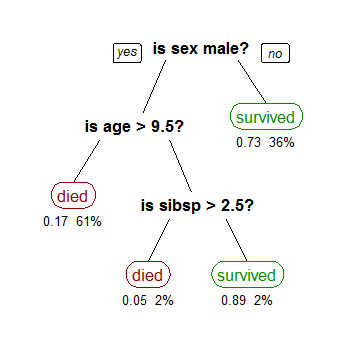
\includegraphics[width=.5\linewidth]{img/randomforest.png}
\caption{Exemple d'arbre de decissió \cite{imgrandomforestregressor}}
\end{figure}

\textit{Random Forest Regressor} \cite{randomforestregressor} és un conjunt d'arbres de regressió, on el resultat és la mitja de la sortida de cada arbre, a més per a cada arbre s'aplica un soroll aleatori a les dades sense variar en la seva distribució, això fa que es benificiï al fer la mitja. 

\newpage

\paragraph{Regressor lineal (LR)}
Un regressor lineal \cite{linearregressor} modelitza una recta de regressió a partir d'un núvol de punts. La recta definida, és la recta més propera que passa per tots els punts. El que busca és definir una variable depenent a partir d'un conjunt de variables, és a dir:
$$
y =\beta_0+\beta_1 x_1+\beta_2 x_2+ \cdots + \beta_n x_n + \varepsilon
$$

on $\beta_i$ són termes constants i $n$ són els conjunts d'observacions que tenim. En el cas d'una sola variable depenent, tindriem un resultat com el de la figura següent:

\begin{figure}[h]
\centering
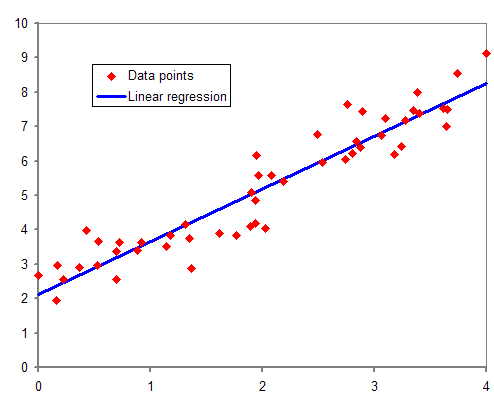
\includegraphics[width=.5\linewidth]{img/linearregression.png}
\caption{Regressió lineal \cite{imglinearregressor}}
\end{figure}

\paragraph{Mètriques utilitzades}
Igual que en la secció de clusterització, per a la predicció de dades, també hem utilitzat mesures per validar les nostres prediccions. Aquí hem utilitzat mesures supervisades. Anomenem $y_{pred}$ al conjunt de qualificacions que s'ha predit d'un alumne, i $y_{test}$ al conjunt de qualificacions real del estudiant.

\subparagraph{Error promig absolut (MAE)}
L'error promig absolut \cite{mae} una mesura supervisada que és basa en fer la mitja dels errors produïts pel predictor. Està definit per la següent fórmula:
$$ \mathrm{MAE} = \frac{1}{n}\sum_{i=1}^n \left| y_{pred_i}-y_{test_i}\right| $$

\subparagraph{Error promig quadràtic (MSE)}
Per un altre banda tenim una segona mètrica, l'error promig quadràtic \cite{mse}, supervisada també. Aquesta mètrica penalitza els error alts, ja que la diferència es elavada al quadrat, quedaria la següent fórmula:
$$\mathrm{MSE}=\frac{1}{n}\sum_{i=1}^n(y_{pred_i}-y_{test_i})^2$$

\subparagraph{Coeficient de pearson (PCC)}
El coeficient de pearson, l'utilitzem com una mètrica supervisada i la fem servir per mesurar la diferencia de la distribució de les notes predites amb les notes reals. El coeficient de pearson està definit per la següent fórmula:
$$\mathrm{PCC} =\left| \frac{\sum_{i=1}^n(y_{pred_i} - \bar{y}_{pred_i})(y_{test_i} - \bar{y}_{test_i})}{\sqrt{\sum_{i=1}^n(y_{pred_i} - \bar{y}_{pred_i})^2  \sum_{i=1}^n(y_{test_i} - \bar{y}_{test_i})^2}}\right|$$

\subparagraph{Desviació estàndard (std)}
També calculem la desviació estàndard per veure si els errors són més o menys dispersos. La fórmula utilitzada és la següent:

$$ \sigma = \sqrt{ \frac{1}{n} \sum_{i=1}^n (\left| y_{pred_i}-y_{test_i}\right| - \mu)^2 } $$

\subparagraph{\textit{Mean Rangking Score (MRS)}}
Aquesta és una técnica desenvolupada per nosaltres, està basada en la mesura de \textit{Error promig absolut}, però amb valors discrets. És una mesura supervisada per tal de mesurar quant de bo és un ranking que s'hagi predit. Es tracta d'una mitja a partir de les distancies d'error en el ranking. La métrica presenta la següent fórmula:

$$ \mathrm{MRS} = \frac{1}{n}\sum_{i=1}^n \left| \gamma(y_{pred_i}) -  \gamma(y_{test_i})\right| $$

on:
\begin{itemize}[leftmargin=.5in]
	\item [$\gamma$] és una funció que ens retorn la posició de l'elemtn en el ranking
\end{itemize}

\newpage

La millor manera d'entendre aquesta mètrica és mostrar un exemple a partir d'aquesta taula:

\begin{table}[h]
\centering
\label{my-label}
\begin{tabular}{@{}cc@{}}
\toprule
Ranking Real & Ranking Predit \\ \midrule
A1           & A4             \\
A2           & A2             \\
A3           & A1             \\
A4           & A3             \\ \bottomrule
\end{tabular}
\caption{Exemple de rankings}
\end{table}

Per aquest exemple, hauriem de recorrer els 4 elements:
	$$\left|\gamma(A1_{notes_r}) - \gamma(A1_{notes_p})\right| = \left| 1 - 3 \right| = 2$$
	$$\left|\gamma(A2_{notes_r}) - \gamma(A2_{notes_P})\right| = \left| 2 - 2 \right| = 0$$
	$$\left|\gamma(A3_{notes_r}) - \gamma(A3_{notes_p})\right| = \left| 3 - 4 \right| = 1$$
	$$\left|\gamma(A4_{notes_r}) - \gamma(A4_{notes_pr})\right| = \left| 4 - 1 \right| = 3$$

Quedant:

$$ \mathrm{MRS} = \frac{2 + 0 + 1 + 3}{4} = \frac{6}{4} = 1.5$$

Ens podem fixar que si comparem dos rankings iguals, llavors $\mathrm{MRS} = 0$. Per tant, com més proper estigui a 0, millor s'aproparà la predicció del ranking real.
\\
\\
Totes aquestes mètriques són necessaries per evaluar cada tècnica de predicció que utilitzo. Tot i així, les tècniques més importants i que tenen més pes són l'error promig absolut i quadràtic.

\subsubsection{Reducció de dimensions}
Una de les últimes tècniques que utilitzo en aquest projecte d'innovació docent és la reducció de dimensions. És imprescindible per poder visualitzar les teves dades si tenen una dimensió major que 3. Aquestes tècniques a més permeten reduïr el cost computacional sense variar en el seu resultat. Una de les tècniques utilitzades en aquest projecte és l'anàlisis de components principals (PCA).

\paragraph{PCA}
L'anàlisis de components principals o PCA \cite{pca} el que fa és escollir un nou sistema de coordenades a partir d'una transformació lineal on s'ordenen les variances per mida. La variança amb major mida s'escollirà com eix principal, la segona variança com a segon eix, així successivament fins obtenir la dimensionalitat escollida per argument.

%http://web.media.mit.edu/~tristan/phd/dissertation/chapter5.html

\newpage

\section{Experiments i resultats}
En aquest apartat s'explicarà pas per pas els resultats obtinguts per cada pregunta plantejada. Fins ara s'han llegit tots els conceptes necessaris per poder entendre aquesta secció de la documentació. Començaré amb les preguntes relacionades amb la clusterització i acabaré amb els resultats obtinguts amb la predicció de notes.
\\
\\
Abans de començar a comentar els resultats, explicaré de quines dades parteixo per respondre cada pregunta. D'inicial tenim tota una taula on cada fila és la qualificació d'un alumne donada un assignatura, per tant en cada fila tenim informació com \textit{l'identificador d'alumne, assignatura, tipus d'apunt (convalidada, ordinaria o de reconeixement), qualificació de l'assignatura,} \ldots És a partir d'aquesta taula que fem una conversió de tal manera que en cada fila ens quedi un alumne i cada columna sigui una assignatura, construint una matriu tal que així:

$$
\bordermatrix{C &         a_1   &    a_2   &   \cdots    &    a_m  \cr
                  e_1    &  c_{11}  &  c_{12}  &   \cdots    &  c_{1m} \cr
                  e_2    &  c_{21}  &  c_{22}  &   \cdots    &  c_{2m}    \cr
                  \vdots &  \vdots  &  \vdots  &   \ddots    &  \vdots \cr
                  e_n    &  c_{n1}  &  c_{n2}  &   \cdots    &  c_{nm} \cr
                  }
$$
on:
\begin{itemize}[leftmargin=.5in]
	\item [$e_i$] és un estudiant.
	\item [$a_i$] és una assignatura.
	\item [$c_{ij}$] és la nota d'un alumne donada una assignatura.
\end{itemize}

$C$ és una matriu amb coeficients reals, $C\in M_{nxn} (\mathbb{R})$ on $0 \leq c_{ij} \leq 10$, és a dir aquesta matriu no conté cap nombre desconegut i que cada alumne $e_i$ ha cursat tot el conjunt d'assignatures $\{a_1, a_2, a_3, \ldots, a_m\}$.
\\
\\
El conjunt d'assignatures que apareixen en les columnes pot variar depenent de la pregunta que volem respondre, pot ser el conjunt d'assignatures de primer, com el conjunt de les de primer més les de segon. Però a partir d'una matriu $C$ com aquesta em basaré algunes qüestions.

\newpage

\subsection{Hi ha diferents perfils d'alumnes?}
La resposta a aquesta pregunta és trobar diferents tipus d'estudiants en relació a la seva nota (alumnes amb notes molt bones en tot, alumnes amb males notes en certes assignatures, alumnes que suspenen, entre altres). Però volem que el nostre algoritme explori els grups que hi han.
\\
\\
Com el que busquem són alumnes amb qualificacions semblants, utilitzarem la tècnica de \textit{K-means}, ja que pot agrupar alumnes en relació a la distància de les seves notes. Però clar, \textit{K-means} té una limitació, necessita com argument el número de clusters que volem segmentar. Hem de trobar una forma de poder trobar la millor $k$.
\\
\\
La primera opció que vam pensar és aplicar \textit{K-means} amb diferents \textit{k} i per cada prova, calcular la mesura de \textit{Silhouette}. L'algoritme de \textit{K-means} rep com a paràmetre una matriu com la matriu $C$ amb els alumnes que hagin cursat totes les assignatures de primer de cada grau implantat en la Facultat de Matemàtiques de la Universitat de Barcelona. 

\begin{figure}[h]
\centering
\begin{subfigure}{.45\textwidth}
  \centering
  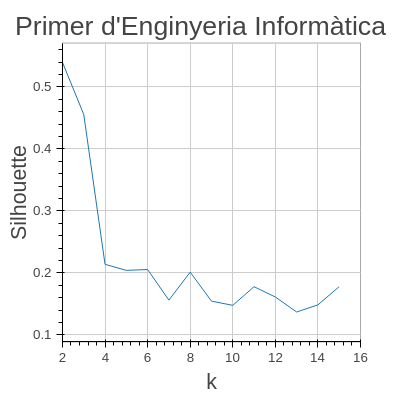
\includegraphics[width=\linewidth]{img/silhouette_primer_info.png}
  \caption{Informàtica}
\end{subfigure}
\begin{subfigure}{.45\textwidth}
  \centering
  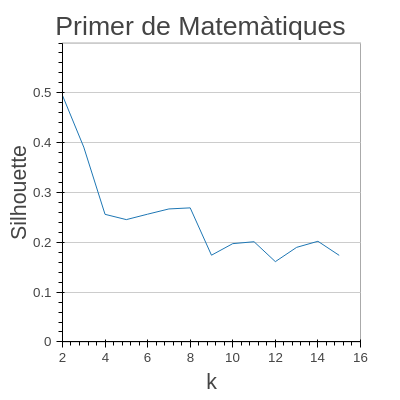
\includegraphics[width=\linewidth]{img/silhouette_primer_mates.png}
  \caption{Matemàtiques}
\end{subfigure}
\caption{Càlcul de la mesura \textit{Silhouette}}
\end{figure}

Aquest gràfic ens diu que la millor $k$ en ambdós casos és $k=2$ i la mesura de silhouette descendeix conforme augmenta el paràmetre $k$. Però clar aquest resultat no ens interesa, perquè busquem un número de clusters major que 2, encara que els clusters estiguin menys disgregats. Per tant com aquesta tècnica no ens serveix hem de buscar una altre forma per determinar quina és la millor $k$.
\\
\\
L'altre solució proposada és reduïr la dimensionalitat de les dades per tal de poder visualitzar-les en un pla dos-dimensional. Per poder fer això podem aplicar la tècnica de PCA per reduïr de 10 dimensions a 2. Un cop visualitzem cada estudiant en un espai 2D, podem aplicar un algoritme d'agrupació com \textit{Mean Shift} per veure quants clusters hi han i poder determinar una $k$ per cada curs.

\begin{figure}[h]
\centering
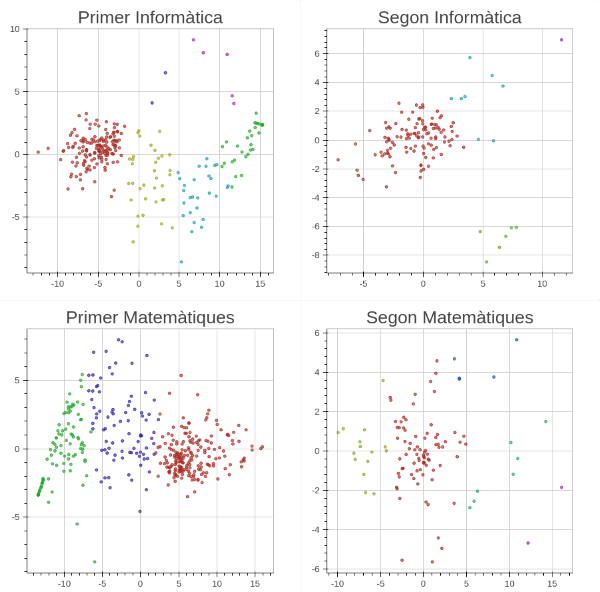
\includegraphics[width=\linewidth]{img/pca_info_mates.png}
\caption{Mean Shift després d'aplicar PCA}
\end{figure}

\newpage

Ara es poden distingir millor el número de clusters o agrupacions que trobem per cada curs.

\subparagraph{Primer d'Enginyeria Informàtica}
Ens separa tot el conjunt de punts en 6 agrupacions (\textit{vermell, beix, blau claret, verd, lila i blau fosc}), però el grup \textit{blau fosc i lila} són un grup tan reduït i separat de la resta que el podriem comptar com un sol cluster. $k=5$

\subparagraph{Segon d'Enginyeria Informàtica}
Per a aquest curs ens separa als estudiants en 4 grups, i podem veure que els clusters estan força disgregats entre ells i no fa falta unificar cap.  $k=4$

\subparagraph{Primer de Matemàtiques} 
Per a primer del grau de Matemàtiques ens separa les observacions en 3 clusters. Com no es veu cap anomalia, a part de la petita separació dels petits punts verds, podem considerar els tres clusters.  $k=3$

\subparagraph{Segon de Matemàtiques}
Aquest és el curs que m'ha donat més problemes, perquè té els punts més distanciats entre ells i això fa que no es pugui interpretar el número de clusters per aplicar \textit{K-means}. Més endavant veurem que el número de clusters òptim és 3, ja que amb 4 ens dóna dos clusters molt semblants, els quals es poden unificar. $k=3$
\\
\\
Ara que ja tenim el valor de $k$ adeqüat per cada curs, podem aplicar la tècnica de \textit{K-means}. S'ha utilitzat una combinació de colors adequada per cada perfil.

\begin{figure}[h]
\centering
\begin{subfigure}{.2\textwidth}
  \centering
  
\includegraphics[width=\linewidth]{img/aprovats.png}
  \caption{Aprovats}
\end{subfigure}
\begin{subfigure}{.2\textwidth}
  \centering
  
\includegraphics[width=\linewidth]{img/bonesnotes.png}
  \caption{Bones notes}
\end{subfigure}
\begin{subfigure}{.2\textwidth}
  \centering
  
\includegraphics[width=\linewidth]{img/suspesos.png}
  \caption{Suspesos}
\end{subfigure}
\begin{subfigure}{.2\textwidth}
  \centering
  
\includegraphics[width=\linewidth]{img/altresperfils.png}
  \caption{Altres}
\end{subfigure}
\caption{Categoria de colors utilitzada per representar els perfils d'estudiants}
\end{figure}

\newpage

Començarem comentant els resultats obtinguts amb el curs de primer d'Enginyeria Informàtica on hem dit que aplicariem \textit{K-means} amb $k=5$.

\begin{figure}[h]
\centering
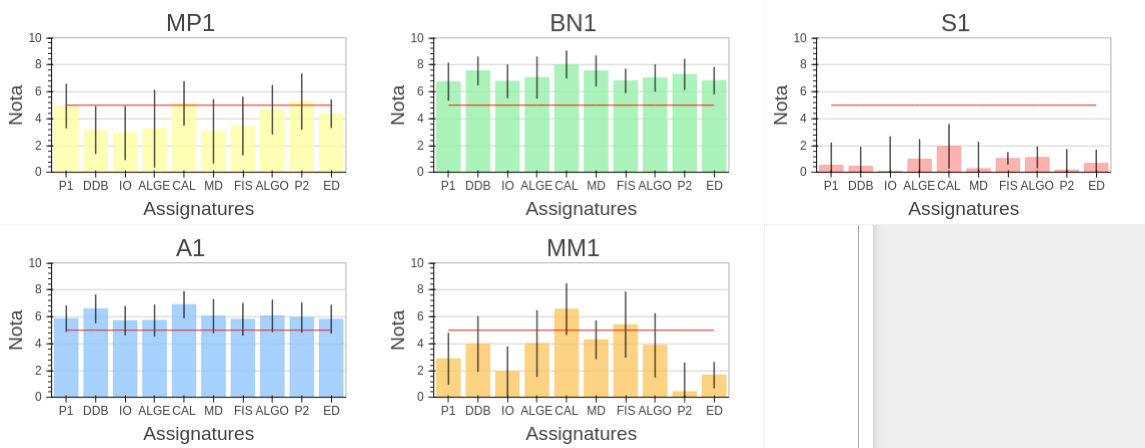
\includegraphics[width=\linewidth]{img/perfils_primer_info.png}
\caption{Perfils d'alumnes de primer d'Enginyeria Informàtica}
\end{figure}

\begin{figure}[h]
\centering
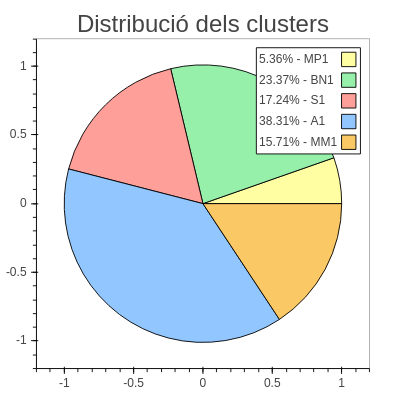
\includegraphics[width=.55\linewidth]{img/perfils_primer_info_pastilla.png}
\caption{Percentatges de cada agrupació}
\label{fig:pasprimerinfo}
\end{figure}

Primer explicaré que és el que veiem en aquests gràfics i així poder interpretar els demés. Cada gràfic són els diferents perfils d'estudiants que ha trobat la tècnica de \textit{K-means}. En cadascun d'ells trobem com a títol l'etiqueta assignada a aquell perfil i el color de cadascún depén de la categoria explicada abans. En l'eix d'abscisses es veuen les assignatures (en aquest cas les de primer d'Enginyeria Informàtica), i en l'eix d'ordenades tenim la mitja de cada assignatura (longitud de la barra). Per últim les línees negres determinen la desviació estàndard de la distribució de cada assignatura i la línea vermella és una marca per identificar l'alçada de l'aprovat.

\subparagraph{MP1 - Millors en programació de primer d'Informàtica} 
Aquest perfil encaixa amb els alumnes que tenen millores notes en les assignatures de programació que en les de Matemàtiques. La distribució d'aquest és molt dispersa, això ho podem veure per la llargada de la barra negra (desviació estàndard). També és, perquè la mostra és petita, representa el 5.36\% de la mostra total.

\subparagraph{BN1 - Bones notes de primer d'Informàtica}
Aquest perfil correspon als alumnes que tenen bones notes en totes les assignatures de primer i com podem veure en el gràfic de pastilla, representen un 23.37\% del total, sent el segon perfil més abundant. Podem veure ara que la mostra és més gran, la desviació estàndard és menor, és a dir, aquest perfil és força estable, tots els estudiants que hi pertanyent es distancien amb una qualificació promig d'1.5 aproximadament.

\subparagraph{S1 - Suspesos de primer d'Informàtica}
Com podem veure, aquest perfil són els estudiants que suspenen la majoria d'assignatures. A primeres podem pensar que són els que solen deixar la carrera i és això el que anem a respondre en la següent pregunta plantejada. També podem veure que són un 17.2 \% del total d'alumnes que han cursat les assignatures de primer, no són un percentatge baix.

\subparagraph{A1 - Aprovats de primer d'Informàtica}
Són la major part dels alumnes, amb un 38.31\% del total, i són els alumnes que de mitja treuen entre 5 i 7. Igual que passa amb el cluster \textit{BN1}, la desviació estàndard de cada assignatura és força baixa, i això fa que el cluster sigui consistent.

\subparagraph{MM1 - Millors en Matemàtiques de primer d'Informàtica}
Aquest perfil igual que \textit{MP1}, és bastant inestable, ja que tenen una desviació estàndard alta, és a dir, hi ha una diversitat de notes elavada, no es concentren tots els alumnes a tenir la mateixa nota. Tot i que siguin dispersos, són un 15.71 \% del total, un percentatge forç alt.
\\
\\
Fent un anàlisis general de les gràfiques, podem veure que en l'assignatura \textit{Estructura de Dades} (ED) presenta sempre una desviació més petita que la resta d'assignatures en cada perfil, és a dir, que les notes en concentren més en la mitja marcada. Per un altre banda també es pot veure que en tots els perfil, sense mirar la qualificació corresponent, la nota més alta en els 6 perfils és de l'assignatura de \textit{Càlcul} (CAL).
\\
\\
Seguint amb l'anàlisis podem veure també els perfils de tots els alumnes que hagin cursat totes les assignatures de segon, on he aplicat \textit{K-means} amb $k=4$.

\begin{figure}[h]
\centering
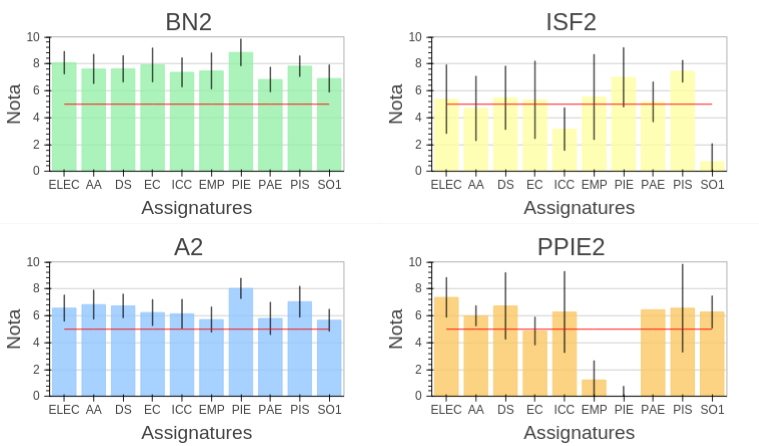
\includegraphics[width=.9\linewidth]{img/perfils_segon_info.png}
\caption{Perfils d'alumnes de segon d'Enginyeria Informàtica}
\end{figure}

\begin{figure}[h]
\centering
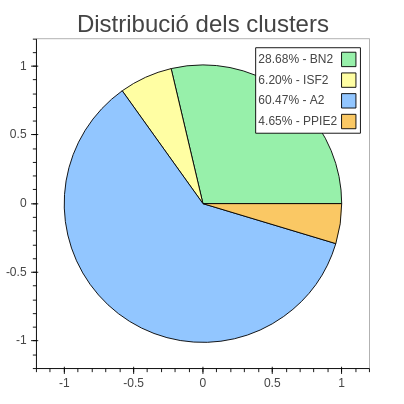
\includegraphics[width=.4\linewidth]{img/perfils_segon_info_pastilla.png}
\caption{Percentatges de cada agrupació}
\end{figure}

\subparagraph{BN2 - Bones notes de segon d'Informàtica}
Aquest és un perfil força semblant a \textit{BN1}, és per això que ens plantejem la pregunta: \textit{Amb quin perfil de provinença encaixa cadascun d'aquests perfils?}, és a dir, és cert que els que tenen bones notes a primer, solen ser els que treuen bones notes a segon, el que anomenem conservació de clusters. De tots els alumnes que han cursat segon un 28.68\% pertanyen a aquest cluster, més d'un quart de la mostra.

\subparagraph{ISF2 - ICC i SO1 fluixes}
Aquest perfil encara que sigui minoritari, amb un 6.2\% del total, és força curiós, ja que són alumnes que tenen \textit{Introducció a la Computació Científica} (ICC) i \textit{Sistemes operatius I} (SO1) amb notes més baixes que la resta. També s'ha de dir que tot i que les mitjes siguin més petites, les desviacions estàndards són molt altes, el que fa que les notes dels alumnes siguin més diverses i no segueixin exactament la distribució de mitjes de cada perfil.

\subparagraph{A2 - Aprovats de segon d'Informàtica}
Aquest perfil és semblant al perfil \textit{A1}, pertany als alumnes que tenen notes entre 5 i 7. Són el 60.47\% del total d'alumnes que han cursat les assignatures de segon.

\subparagraph{PPIE2 - Problemes amb PIE i Empresa}
Aquest és el perfil amb un percentatge més petit de població, un 4.65\%. És un perfil força dispers, ja que les desviacions estàndar són altes, i això es pot veure en assignatures com PIS o ICC. A més és curiós perquè és un grup que apareixen amb \textit{Empresa} (EMP) i \textit{Probabilitat i estadística} (PIE) suspeses, però no he trobat un perquè a aquest fenòmen.
\\
\\
Ens podem fixar que la distribució de mitjes del perfil \textit{BN2} i \textit{A2}, és força semblant, només que \textit{BN2} té les mitjes més altes.
\\
\\
Deixant enrere al grau d'Enginyeria Informàtica, em poso a analitzar als estudiants del grau en Matemàtiques. Comencem amb els alumnes de primer, els quals els segmentem en 3 agrupacions ($k=3$).

\newpage

\begin{figure}[h]
\centering
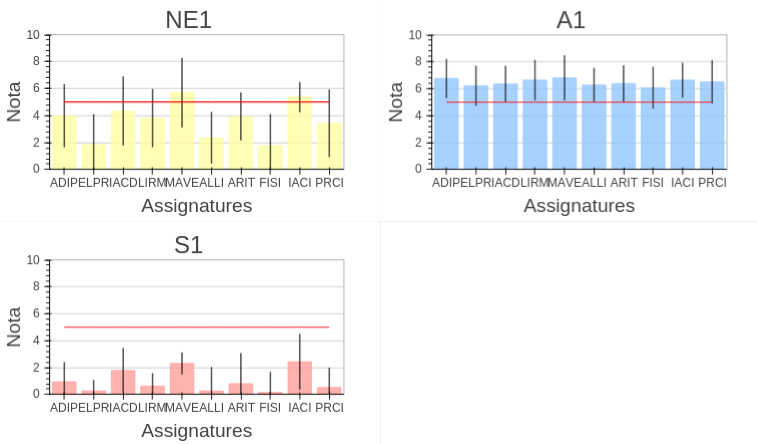
\includegraphics[width=.9\linewidth]{img/perfils_primer_mates.png}
\caption{Perfils d'alumnes de primer de Matemàtiques}
\end{figure}

\begin{figure}[h]
\centering
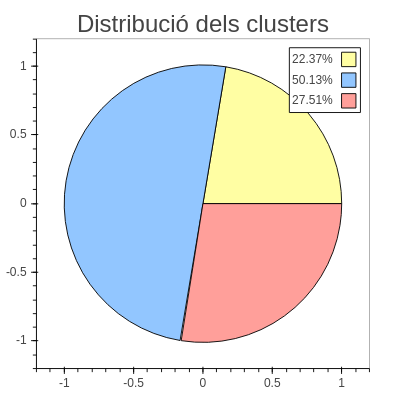
\includegraphics[width=.4\linewidth]{img/perfils_primer_mates_pastilla.png}
\caption{Percentatges de cada agrupació}
\end{figure}

\subparagraph{NE1 - No estables de primer de Matemàtiques}
Podem veure que aquest cluster té les mostres molt distanciades, per les desviacions estàndards que presenta. Aquest perfil l'he classificat com \textit{No estables de primer}, ja que són alumnes que amb prou feines poden aprovar certes assignatures. Conformen un 22.37\% del total d'alumnes.

\subparagraph{A1 - Aprovats de primer de Matemàtiques}
Aquest perfil pertany als estudiants que tenen totes les assignatures aprovades  de mitja i són els que formen la major part del total, amb un 50.13\%.

\subparagraph{S1 - Suspesos de primer de Matemàtiques}
Per últim, i sense faltar, tenim els alumnes que de mitja suspenen totes les assignatures. Conformen un 27.51\% del total d'estudiants.
\\
\\
Els resultats són força esperats per aquest curs, tenim els que ho aproven tot i els que ho suspenen tot, i per un altre banda tenim la resta que no pertanyen ni a un ni a l'altre.
\\
\\
Per últim tenim als alumnes de segon de Matemàtiques, on no s'observa res interessant com tenim als perfils de Informàtica.

\begin{figure}[h]
\centering
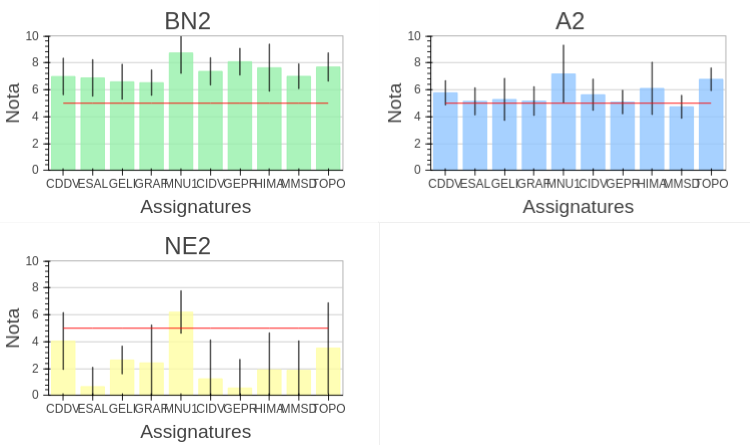
\includegraphics[width=.85\linewidth]{img/perfils_segon_mates.png}
\caption{Perfils d'alumnes de segon de Matemàtiques}
\end{figure}

\begin{figure}[h]
\centering
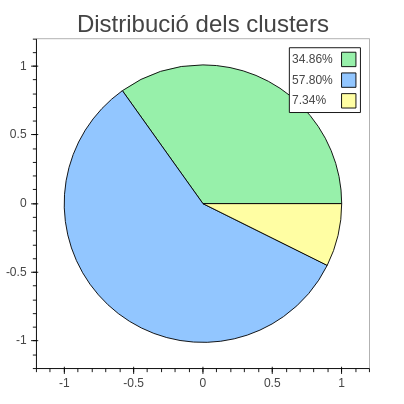
\includegraphics[width=.4\linewidth]{img/perfils_segon_mates_pastilla.png}
\caption{Percentatges de cada agrupació}
\end{figure}

\newpage

\subparagraph{BN2 - Bones notes de segon de Matemàtiques}
Torna a aparèixer aquest tipus de perfils, alumnes amb mitjes de qualificacions altes. Tot i així, és sorprenent el percentatge d'alumnes que pertanyen a aquest cluster, un 34.86\%.

\subparagraph{A2 - Aprovats de segon de Matemàtiques}
Per un altre banda tornem a tenir els alumnes amb qualificacions en el rang d'aprovat, tot i que la majoria freguen la línea de l'aprovat, com és en tots els casos, aquest és el perfil més abundant, amb un 57.80\%.

\subparagraph{NE2 - No estables de segon de Matemàtiques}
Igual que a primer del grau de Matemàtiques tenim el perfil de \textit{No estables}, aquí el tornem a tenir, tot i que aquest perfil només té aprovada per mitja una assignatura, \textit{Mètodes numèrics I} (MNU1). Pertanyen al 7.34\% del total.
\\
\\
En aquest curs tenim un efecte semblant a primer d'Enginyeria Informàtica amb l'assignatura de \textit{Càlcul}, hi ha una assignatura que en tots els perfils té la mitja més alta, \textit{Mètodes numèrics I} (MNU1).

\newpage

\subsection{Quina és la tassa d'abandonament per cada tipus de perfil?}
És cert que els que suspenen abandonen la carrera? Ara ho podrem demostrar amb gràfics estadístics. Ens centrarem en la tassa d'abandonament dels alumnes que cursen primer, tant d'Enginyeria Informàtica com el grau de Matemàtiques. Tornaré a mostrar els perfils per poder discutir cada perfil amb la seva tassa d'abandonament.

\begin{figure}[h]
\centering
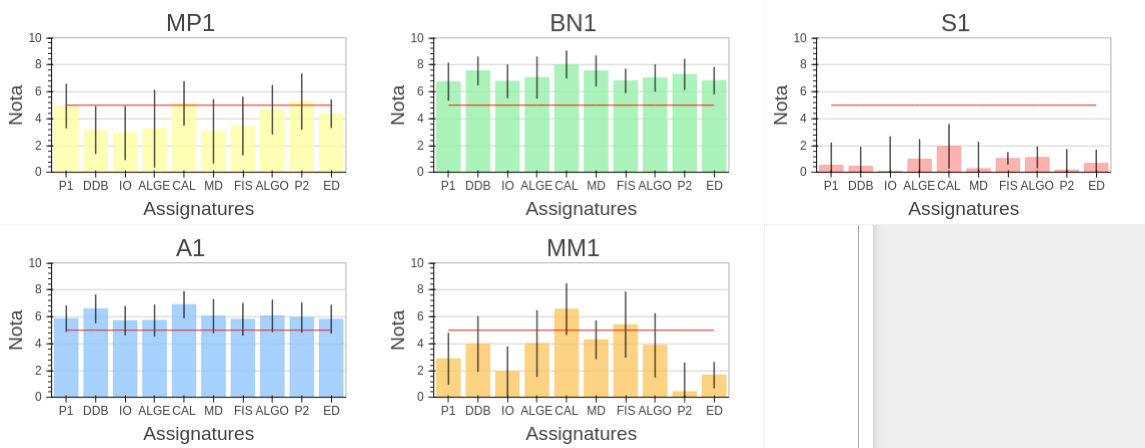
\includegraphics[width=\linewidth]{img/perfils_primer_info.png}
\caption{Perfils d'alumnes de primer d'Enginyeria Informàtica}
\end{figure}

\begin{figure}[h]
\centering
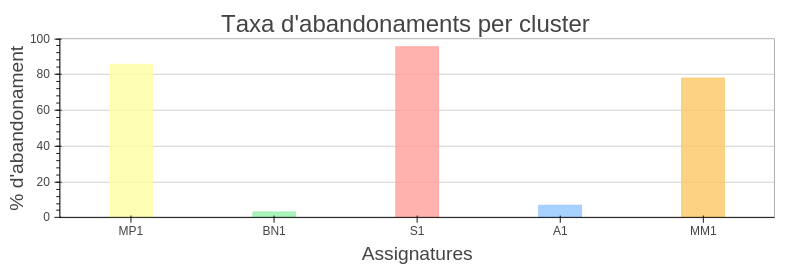
\includegraphics[width=\linewidth]{img/abandonaments_primer_info.png}
\caption{Tassa d'abandonaments per perfil}
\label{fig:abandonamentprimer}
\end{figure}

Els alumnes que amb més probabilitat deixen la carrera són els que suspenen, seguits d'estudiants que no tenen unes notes massa estables. És a dir, que la majoria que passen a segon pertanyen al cluster \textit{BN1} i \textit{A1}. Però si ens fixem una mica en el gràfic d'abandonaments, els perfils d'aprovats i de bones notes, hi ha un petit percentatge indicat que diu que abandonen la carrera. En les dades que tenim, no tenim un camp que ens indiqui si un alumne ha abandonat la carrera o no, ja que no ho tenen registrat. Hem hagut d'agafat per cada perfil tot el conjunt d'alumnes d'aquell perfil i s'ha comprovat per cadascún si té assignatures matriculades a l'any següent. Però clar, hi han alumnes del darrer any que s'han de matricular per l'any vinent encara (i no apareixen matriculats a l'any següent), per això hi ha un petit marge d'error i els clusters \textit{BN1} i \textit{A1} aparèixen amb una mínima tassa d'abandonaments. 
\\
\\
Per altre banda tenim el curs de primer de Matemàtiques, on apliquem el mateix algoritme explicat en el paràgraf anterior. També trovem un petit marge d'error en els perfils que ho aproven tot.

\begin{figure}[h]
\centering
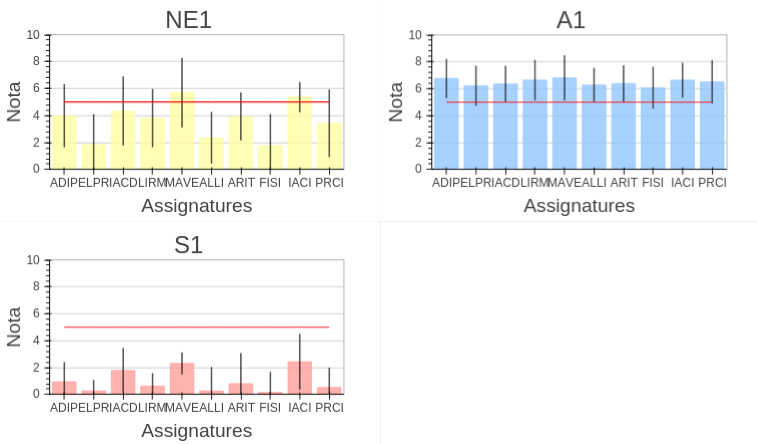
\includegraphics[width=\linewidth]{img/perfils_primer_mates.png}
\caption{Perfils d'alumnes de primer d'Enginyeria Informàtica}
\end{figure}

\begin{figure}[h]
\centering
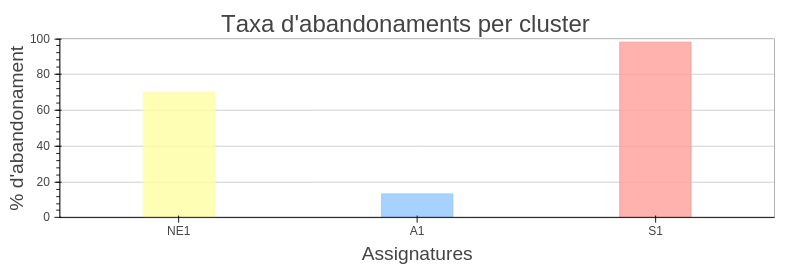
\includegraphics[width=.9\linewidth]{img/abandonaments_primer_mates.png}
\caption{Tassa d'abandonaments per perfil}
\end{figure}

Igual que en Enginyeria Informàtica, ens trobem que la major tassa d'abandonament es troba en els alumnes que suspenen per mitja totes les assignatures. Seguidament els hi segueixen els estudiants que no tenen unes notes massa regulars i com s'ha comentat anteriorment, els alumnes que estan classificats com \textit{Aprovats}, també surten amb una tassa mínima d'abandonament.

\subsection{Amb quin perfil de provinença encaixa cadascun d'aquests perfils?}
El que es vol mirar en aquesta pregunta és la conservació de clusters, per exemple, els estudiants que treuen bones notes a primer, segueixen treien bones notes a segon? O, de quina via d'accés solen provenir els estudiants de primer de Matemàtiques? Preguntes com aquestes anem a resoldre en aquest apartat. 
\\
\\
Començarem, com hem fet anteriorment, amb els estudiants que han cursat primer d'Enginyeria Informàtica. Com s'ha explicat en la secció de preguntes plantejades, contrastem primer d'Enginyeria Informàtica amb les vies d'accés: Batxillerat i salt d'Universitat.

\todo{Canviar els colors de la gràfica si dóna temps}
\begin{figure}[h]
\centering
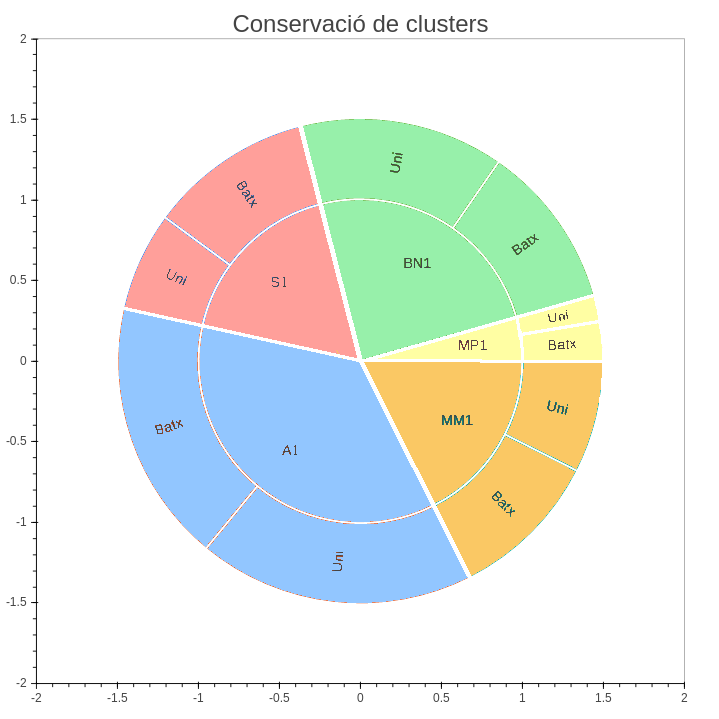
\includegraphics[width=.6\linewidth]{img/conservacio_clusters_primer_info.png}
\caption{Conservació de clusters dels alumnes de primer d'Informàtica}
\end{figure}

En l'interior del cercle, podem veure el mateix gràfic de pastilla que s'ha vist anteriorment dels perfils dels estudiants de primer d'Enginyeria Informàtica [fig:~\ref{fig:pasprimerinfo}]. Per fóra del cercle de cada perfil es veu quantitativament d'on venen els alumnes del perfil. 
\\
\\
Es pot veure com en tots els perfils, venen meitat de Batxillerat i meitat de Salt d'Universitat aproximadament. Es pot distingir que els estudiants classificats com \textit{Suspesos} solen venir més de Batxillerat que no pas d'una altre Universitat, tot i que la diferència és petita. Com s'ha vist en la gràfica d'abandonament [fig:~\ref{fig:abandonamentprimer}], els alumnes que passen amb més abundancia a segon són els classificats com \textit{A1} i \textit{BN1}, per tant procedim a eliminar a la resta, ja que són minoria, i així més llegible la següent gràfica.

\begin{figure}[h]
\centering
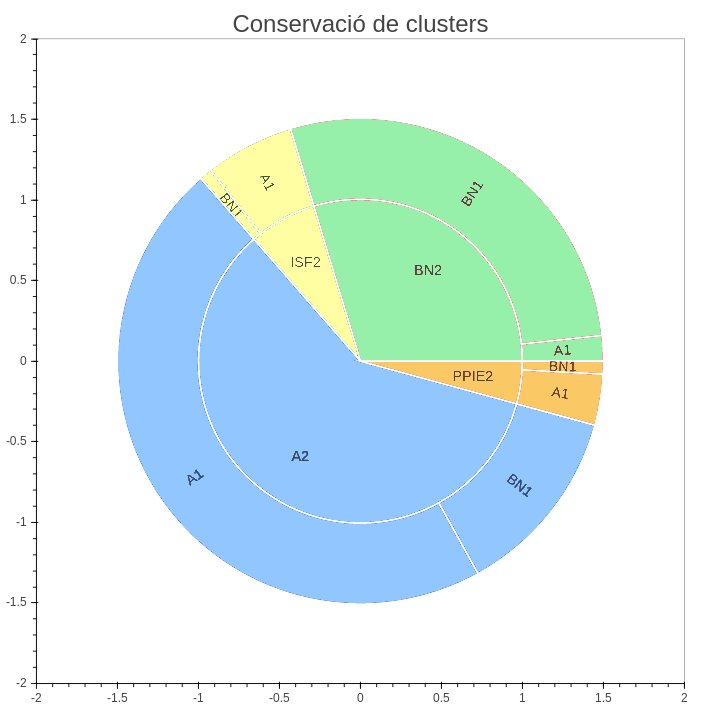
\includegraphics[width=.6\linewidth]{img/conservacio_clusters_segon_info.png}
\caption{Conservació de clusters dels alumnes de primer d'Informàtica}
\end{figure}

Ara és veu amb més claredat el significat d'un gràfic com aquest, ja que podem veure com els que solen treure bones notes a primer d'Enginyeria Informàtica, solen treure bones notes a segon també, i els que es classificaven com \textit{Aprovats de primer}, solen parar a \textit{Aprovats de segon}. També podem veure com un petit percentatge d'alumnes que treuen notes a primer, passen a treure notes més baixes a segon, igual que alumnes etiquetats com \textit{Aprovats de primer} amb una petit quanitat paren a perfils inestables com \textit{ISF2} o \textit{PPIE2}.

\newpage

Per últim es veurà la provinença dels estudiants de primer del grau de Matemàtiques, on també es pot veure una tendencia.

\begin{figure}[h]
\centering
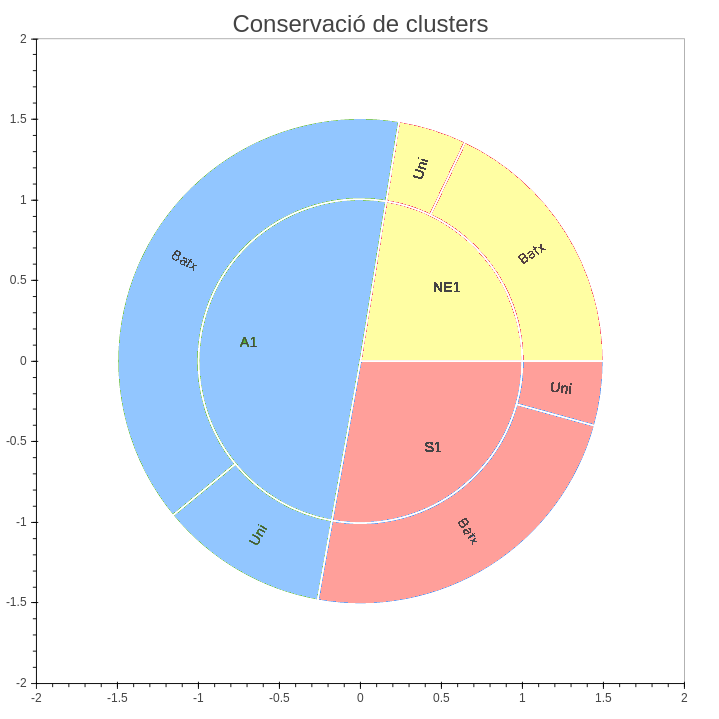
\includegraphics[width=.6\linewidth]{img/conservacio_clusters_primer_mates.png}
\caption{Conservació de clusters dels alumnes de primer d'Informàtica}
\end{figure}

En aquesta gràfica es veu amb claredat que la major part d'estudiants que han cursat primer del grau de Matemàtiques, venen de Batxillerat. 

Una de les raons per les quals vam plantejar aquesta pregunta, era per saber si podiem determinar un perfil d'estudiant al grau a partir de la via d'accés d'aquest. Malauradament no s'ha trobat cap correlació com aquesta, però s'han pogut veure resultats molt coherents i que no esperavem trobar.

\newpage

\subsection{Predicció de notes i ranking de dificultat d'assignatures}
Per últim en aquest apartat s'explicará  les tècniques de predicció que hem fet servir i quins resultats, tant quantitatius com qualitatius, s'han obtingut. La resposta que busquem d'aquesta pregunta, és poder mostrar un ranking, personalitzat per cada alumne, d'assignatures ordenades per la dificultat (és a dir, per notes) que li pot arribar a costar a cada estudiant.
\\
\\
Abans de construïr el ranking, necessitem saber quina és la tècnica de predicció que s'ajusta millor a les nostres dades. Les técniques utilitzades per aquest experiment han sigut les següents, ja anteriorment explicades:

\begin{itemize}[leftmargin=.5in]
	\item Recomanador col·laboratiu bassat en estudiant
	\item Recomanador col·laboratiu bassat en assignatures
	\item \textit{Random Forest Regressor}
	\item Regressor lineal
\end{itemize}

El primer pas és la construcció d'un recomanador col·laboratiu, com l'explicat a la secció de Recomanadors, seguint l'interfaç dels predictors de la biblioteca informàtica de \textit{Scikit-learn}. Un predictor en \textit{sklearn} ha de tenir un mètode \textit{fit} i un altre que sigui \textit{predict}. En la següent figura es pot veure el fluxe de les crides a les funcions.

\begin{figure}[h]
\begin{minted}
[
framesep=5mm,
baselinestretch=1.2,
bgcolor=bgcode,
fontsize=\footnotesize
]
{python}
from sklearn.linear_model import LinearRegression
# Definim les variables
X = [(1,2,3), (5,3,2), (3,1,0), (123,433,452), (233,231,786)]
# Fem el promig per cada Xi
y = [2, 3.33, 1.33, 336, 416]
# Definim una nova variable
x = (45,34,65) # promig = 48
# Creem un predictor
predictor = LinearRegression()
predictor.fit(X,y)
print predictor.predict(x)
# >> 47.9271056831
\end{minted}
\caption{Fluxe de crides de funcions d'un predictor d'sklearn}
\end{figure}

\newpage

Primer s'ha de cridar al mètode \textit{fit} i seguidament ja podem cridar al mètode \textit{predict} tantes vegades com volguem per predir.

\begin{figure}[h]
\begin{minted}
[
framesep=5mm,
baselinestretch=1.2,
bgcolor=bgcode,
fontsize=\footnotesize
]
{python}
class Recomender(BaseEstimator):
    def __init__(self, method=coefPearson, transpose=False):
        self._m = None
        self._method = method
        self._transpose = transpose
        
    def fit(self, X, y):
        # ...
        return self
    
    def predict(self, X):
        # ...
        return predicted
\end{minted}
\caption{Estructura del recomanador col·laboratiu}
\end{figure}

Aquesta és la estructura del recomanador col·laboratiu que s'ha construït seguint les fórmules explicades en la secció de Recomanadors. El constructor accepta per paràmetre la funció de similitud entre items (per defecte el coeficient de pearson), i un boleà que determina si és un Recomanador col·laboratiu basat en alumnes (\textit{transpose=False}) o un Recomanador col·laboratiu basat en assignatures (\textit{transpose=True}).
\\
\\
Un cop ja tenim llest tots els predictors, anem a mesurar quantitativament quin dels 4 predictors s'adequa més a les nostres dades. Les mètriques que s'utilitzaran són les que ja s'han explicat en la secció de \textit{Mètriques de predictors}.

\paragraph{Proves quantitatives}
Totes les proves realitzades s'han fet a partir de les notes d'Enginyeria Informàtica. Les proves es basen en dividir les dades en \textit{training} i \textit{test}. \textit{Training} és el conjunt de dades que fem servir per entrenar el predictor (a través de la funció \textit{fit}). \textit{Test} és el conjunt de dades que utilitzem per predir (funció \textit{predict}) i així comprovar si el predictor és lo suficient bo o no. Les proves s'han realitzat a partir de dos conjunts diferents de dades:

\begin{itemize}[leftmargin=.5in]
	\item Una on s'aplica com a \textit{training} les notes de primer d'Enginyeria Informàtica i com a \textit{test} les notes de segon.
	\item Per un altre banda s'ha aplicat un \textit{training} amb les notes de primer i segon, i un \textit{test} amb les notes de tercer d'Enginyeria Informàtica.
\end{itemize}

Per cada una de les proves s'han realitzat diferents proves, que són les següents:

\subparagraph{Proves amb dades continues}
Provem els predictors mirant l'error produït amb les notes real i les predites qualificades del 0 al 10. Les mesures utilitzades en aquesta prova són:

\begin{itemize}[leftmargin=.5in]
	\item \textbf{Error Promig Absolut} Per calcular la diferència mitja d'error produït.
	\item \textbf{Error Promig Quadràtic} Per veure si els errors són molt elevats.
	\item \textbf{Coeficient de Pearson} Per veure si la distribució entre les notes es manté.
	\item \textbf{Desviació estàndard} Utilitzada per veure si els errors es concentren o estan molt disgregats.
\end{itemize}

A més a partir dels errors produïts per cada predictor, es mostra un diagrama de caixes \cite{boxplot} per representar la distribució dels errors. Més endavant amb un dels resultats s'explicarà l'interpretació del diagrama de caixes. Utilitzem un 90\% de \textit{training} i un 10\% de \textit{test}.


\subparagraph{Proves amb dades discretes}
Igual que comprovem l'error produïr amb valors continus, del 0 al 10, ara etiquetem les notes segons el seu rang. El rang que s'ha utilitzat és el següent:

\begin{itemize}[leftmargin=.5in]
	\item \textbf{Suspés} Notes inferiors a 5 ($nota < 5$)
	\item \textbf{Aprovat} Notes entre 5 i 7 ($5 \leq nota < 7 $)
	\item \textbf{Notable} Notes entre 7 i 9 ($7 \leq nota < 9 $)
	\item \textbf{Excel·lent} Notes superiors a 9 ($nota \geq 9$)
\end{itemize}

Per poder visualitzar aquesta prova s'ha utilitzat una matriu de confusió \cite{confusionmatrix}, on es representa amb un mapa de color (o heatmap). En la següent secció s'explicarà que és un mapa de color juntament amb els resultats obtinguts. S'utilitza un 50\% de \textit{training} i un 50\% de \textit{test}.

\subparagraph{Proves amb ranking d'assignatures}
Per últim tenim les proves realitzades per mesurar el ranking que volem desenvolupar. La mètrica utilitzada ha sigut la \textit{Mean Ranking Score}, que com ja s'ha explicat anteriorment, és una mètrica que ens permet mesurar quant de bó és un ranking.

\paragraph{Resultats de les proves quantitatives}
Comançarem amb les proves fetes amb dades continues amb els dos conjunt de dades que s'han explicat en l'apartat anterior.  Utilitzem un 90\% de \textit{training} i un 10\% de \textit{test}.

\begin{figure}[h]
\centering
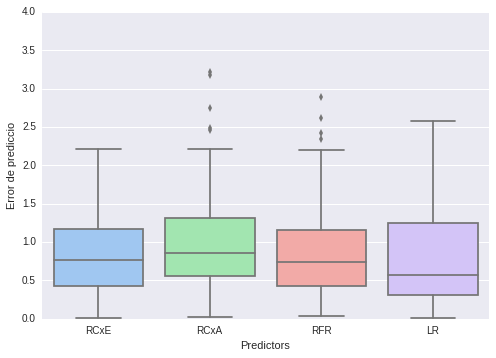
\includegraphics[width=.7\linewidth]{img/boxplot_primer_segon.png}
\caption{Prova amb dades continues. Traning: primer}
\end{figure}

En aquesta figura podem veure un diagrama de caixes, aquest tipus de diagrama representa visualment una distribució. Cada caixa té les mateixes característiques: la línea del centre representa la mediana de la distribució, la caixa es visualitza un 50\% de la mostra (des del primer quartil, fins al tercer), les línes verticals determinen el límit de les distribucions i per últim tota mostra que estigui fóra de lo normal (mostra atípica) és visualitza per fóra dels límits amb un punt.
\\
\\
La distribució que podem veure a la figura són els errors que es presenten en cada predicció, pertant un predictor perfecte, mostrarà una distribució uniforme en el 0. En la figura es pot veure els quatre predictors utilitzats i quina distribució d'error segueix cadascún. Veiem que el predictor més estable i que concentra millor els errors són el recomanador col·laboratiu basat en estudiant i el \textit{random forest regressor}. Per un altre banda tenim el regressor lineal que presenta la mediana més baixa, tot i que el tercer quartil és massa elevat. Els \textit{outlayers}  (mostres atípiques) que veiem tenen una explicació. Què passa si un alumne té un imprevist i no pot cursar una assignatura ja matrículada? Aquest factor no el contemplen els predictors. És per això que tenim observacións atípiques, perquè els predictors potser prediuen que un alumne treurà un 7, però l'alumne per qualsevol raó es desmatricula de l'assignatura, llavors en aquella assignatura li queda un 0. Més avall es mostra un exemple d'una mostra atípica amb una prova qualitativa.

Les mateixes conclusions podem extreure de les mètriques que utilitzem per fer aquesta prova:

\begin{table}[h]
\centering
\begin{tabular}{lllll}
\hline
\textit{\textbf{Algoritme$\setminus$Mètriques}} & \textbf{MAE} & \textbf{MSE} & \textbf{PCC} & \textbf{std} \\ \hline
\textbf{RCxE}          & 0.796          & 0.910          & 0.578          & 0.526          \\
\textbf{RCxA}          & 1.006          & 1.509          & 0.309          & 0.705          \\
\textbf{RFR}           & 0.868          & 1.152          & 0.505          & 0.632          \\
\textbf{LR}            & 0.809          & 1.071          & 0.575          & 0.646          \\ \hline
\end{tabular}
\caption{Mètriques per a proves quantitatives amb dades continues. Traning: primer}
\end{table}

Observem amb les mètriques que els millors predictors són RCxE, RFR i LR, tot i el que presenta menys errors és RCxE ja que té el l'error promig quadràtic més baix.

Igual que hem fet proves amb les notes de primer com a \textit{training} i les de segon com a \textit{test}, ara visualitzarem els mateixos resultats, però com a \textit{training} tenim les notes de primer juntament amb les de segon i com a \textit{test} les notes de tercer.

\begin{figure}[h]
\centering
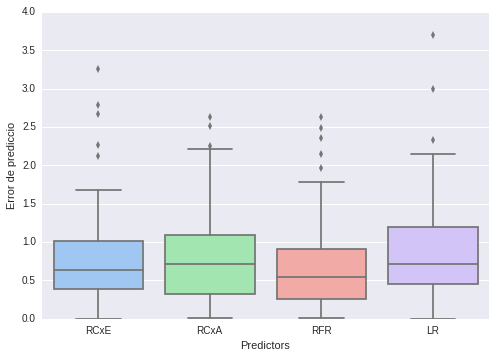
\includegraphics[width=.7\linewidth]{img/boxplot_primersegon_tercer.png}
\caption{Prova amb dades continues. Traning: primer i segon}
\end{figure}

\begin{table}[h]
\centering
\begin{tabular}{lllll}
\hline
\textit{\textbf{Algoritme$\setminus$Mètriques}} & \textbf{MAE} & \textbf{MSE} & \textbf{PCC} & \textbf{std} \\ \hline
\textbf{RCxE}          & 0.869          & 1.590          & 0.276          & 0.914          \\
\textbf{RCxA}          & 0.906          & 1.781          & 0.141          & 0.980          \\
\textbf{RFR}           & 0.786          & 1.522          & 0.339          & 0.951          \\
\textbf{LR}            & 0.932          & 1.890          & 0.283          & 1.011          \\ \hline
\end{tabular}
\caption{Mètriques per a proves quantitatives amb dades continues. Traning: primer i segon}
\end{table}

En aquestes proves podem seguir veient com els millors predictors són el RCxE i el RFR, tot i que ara ambdós presenten més mostres atípiques. Les distribucions i els resultats són semblants als resultats provats amb les dades anteriors. L'únic predictor que marca més diferència és el Random Forest Regressor, ja que disminueix força  la mediana de la distribució, i l'error promig absolut.

\newpage

Ara passem a veure els resultats que s'han obtingut amb les notes discretes (suspés, aprovat, notable i excel·lent). Com ja s'ha explicat, la representació d'aquestes proves es fa amb una matriu de confusió, seguidament paso a descriure que representa.

\begin{figure}[h]
\centering
\begin{subfigure}{.48\textwidth}
  \centering
  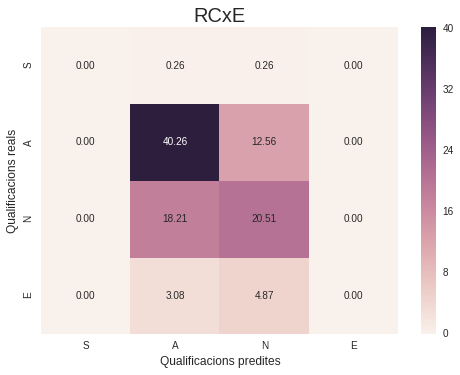
\includegraphics[width=\linewidth]{img/heatmap_rcxe_primer_segon.png}
  \caption{RCxE}
\end{subfigure}
\begin{subfigure}{.48\textwidth}
  \centering
  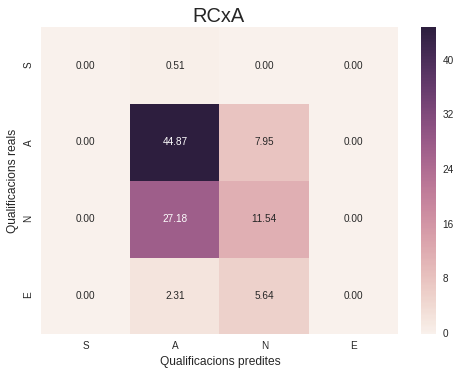
\includegraphics[width=\linewidth]{img/heatmap_rcxa_primer_segon.png}
  \caption{RCxA}
\end{subfigure}
\end{figure}
\begin{figure}[h]
\centering
\begin{subfigure}{.48\textwidth}
  \centering
  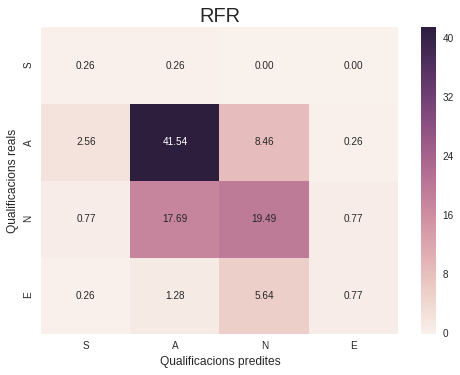
\includegraphics[width=\linewidth]{img/heatmap_rfr_primer_segon.png}
  \caption{RFR}
\end{subfigure}
\begin{subfigure}{.48\textwidth}
  \centering
  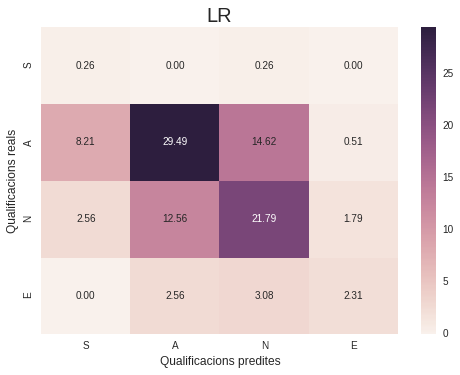
\includegraphics[width=\linewidth]{img/heatmap_lr_primer_segon.png}
  \caption{LR}
\end{subfigure}
\caption{Matriu de confusió. Training: primer}
\end{figure}

En cada matriu de colors podem veure 16 caselles, cada fila i columna posa: S, A, N i E, que significa: suspés, aprovat, notable i excel·lent. Cada cel·la significa el percentatge de vegades que la qualificació predita coincideix amb la qualificació real corresponent. Possem un exemple per acabar d'entendre, en la primera figura apareix en la correspondència de aprovats amb aprovats un 40.26\%, això significa que el 40.26\% de les proves diu el predictor que un alumne treurà una nota d'aprovat i la nota real és aprovat. Si ens fixem com més alt sigui el percentatge, més fosca és la casella. Per tant el que busquem és tenir fosca la diagonal, ja que vol dir que ha encertat tot. Ho representem amb aquest tipus de representació perquè equivocar-se de suspés a aprovat és acceptable, però no de suspés a excel·lent, és per això que s'ha de veure una tendencia de color a les rodalies de la diagonal.
\\
\\
Podem veure que els millors predictors són els recomanadors, ja que mantenen força alta la intensitat de color de la diagonal i el color fosc es manté força concentrat a la diagonal. Si ens fixem en el \textit{Random Forest Regressor} i en el \textit{Regressor lineal} confon més per les seves rodalies. En canvi trobem que tots els predictos confonen aprovats per excel·lents.
\\
\\
Per un altre banda també s'ha provat amb \textit{training} les notes de primer juntament amb les de segon i com a \textit{test} les notes de tercer.

\begin{figure}[h]
\centering
\begin{subfigure}{.42\textwidth}
  \centering
  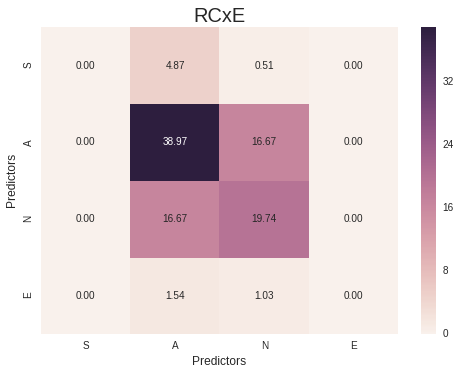
\includegraphics[width=\linewidth]{img/heatmap_rcxe_primersegon_tercer.png}
  \caption{RCxE}
\end{subfigure}
\begin{subfigure}{.42\textwidth}
  \centering
  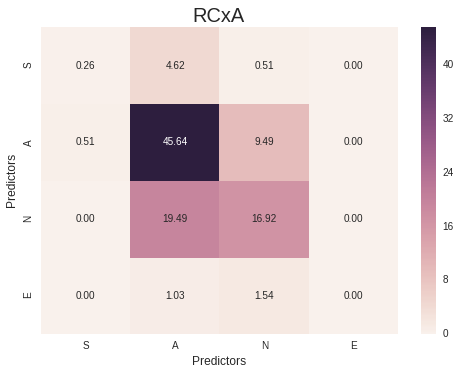
\includegraphics[width=\linewidth]{img/heatmap_rcxa_primersegon_tercer.png}
  \caption{RCxA}
\end{subfigure}
\end{figure}
\begin{figure}[h]
\centering
\begin{subfigure}{.42\textwidth}
  \centering
  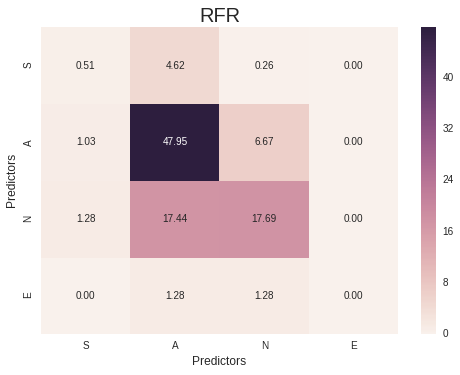
\includegraphics[width=\linewidth]{img/heatmap_rfr_primersegon_tercer.png}
  \caption{RFR}
\end{subfigure}
\begin{subfigure}{.42\textwidth}
  \centering
  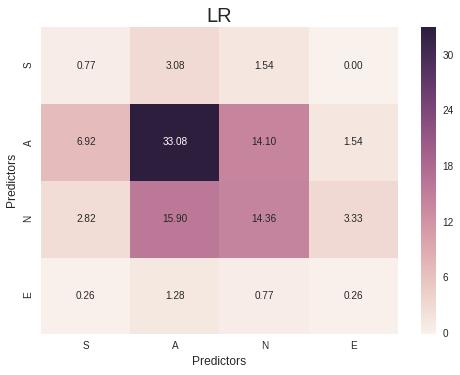
\includegraphics[width=\linewidth]{img/heatmap_lr_primersegon_tercer.png}
  \caption{LR}
\end{subfigure}
\caption{Matriu de convulsió. Training: primer i  segon}
\end{figure}

En aquesta figura es pot veure com RCxE, RCxA i RFR tenen resultats semblants, però en canvi veiem que el regressor lineal es dispersa molt i sol fer fallos amb un salt de dos categories, com per exemple confondre notables amb suspesos. Tot i així, tots ells concentren força bé els resultats a la diagonal.
\\
\\
Per finalitzar la part de proves quantitatives, ens queda fer les proves per al ranking d'assignatures. Per això s'ha utilitzat, com ja s'ha explicat, la mesura de \textit{Mean Ranking Score} per avaluar la qualitat de cada predictor i veure quin predictor és més bo per fer un ranking. Els resultats obtinguts són purament numèrics i venen representats en la següent taula:

\begin{table}[h]
\centering
\begin{tabular}{@{}ccccc@{}}
    & \rotatebox{90}{RCxE} & \rotatebox{90}{RCxA} & \rotatebox{90}{RFR} & \rotatebox{90}{LR} \\ \midrule
MRS & 2.05                   & 2.975                   & 2.2                  & 1.975                 \\ \bottomrule
\end{tabular}
\caption{Mean Ranking Score. Training: primer}
\end{table}

\begin{table}[h]
\centering
\begin{tabular}{@{}ccccc@{}}
    & \rotatebox{90}{RCxE} & \rotatebox{90}{RCxA} & \rotatebox{90}{RFR} & \rotatebox{90}{LR} \\ \midrule
MRS & 2.375                   & 3.4                   & 2.375                  & 2.525                 \\ \bottomrule
\end{tabular}
\caption{Mean Ranking Score. Training: primer i segon}
\end{table}

Es poden veure els resultats de les dues proves (amb diferents \textit{training}) juntes per poder-les discutir. Recordem que la mesura MRS és una mesura que com més propera a 0, millor. Si ens fixem els valors són més baixos a la primera taula, i el millor predictor per aquesta és el recomanador col·laboratiu basat en l'estudiant. On el \textit{training} es fa amb les notes de primer i segon podem veure que els millors predictors són RCxE i RFR.

\newpage

\paragraph{Proves qualitatives}
Un cop hem fet les proves quntitatives i s'ha observat quin predictor és millor per cada cas, passem a utilitzar el millor predictor per veure un cas d'èxit i un de fracàs. En aquest apartat mostraré un cas d'èxit i de fracàs per fer una recomanació de notes, i seguidament un cas d'èxit i fracàs del ranking d'assignatures.
\\
\\
En les proves quantitatives, hem pogut veure que el millor predictor per predir notes quantitatives (de 0 a 10) és el recomanador col·laboratiu basat en l'estudiant. És per això que utilitzarem aquest predictor per fer les proves qualitatives.

% cas d'èxit nota quantitativa
% possar una taula com la de les hores de dedicació
% possar una taula comparant les notes predites amb les reals
\begin{table}[h]
\centering
\begin{tabular}{@{}ccccccccccc@{}}
      & \rotatebox{90}{P1} & \rotatebox{90}{DDB} & \rotatebox{90}{IO} & \rotatebox{90}{ALGE} & \rotatebox{90}{CAL} & \rotatebox{90}{MD} & \rotatebox{90}{FIS} & \rotatebox{90}{ALGO} \ & \rotatebox{90}{P2}& \rotatebox{90}{ED} \\ \midrule
Notes & 7.40 & 8.00 & 6.80 & 6.80 & 6.80 & 7.90 & 6.80 & 7.60 & 7.30 & 9.00 \\ \bottomrule
\end{tabular}
\caption{Notes reals de primer del primer cas d'èxit}
\end{table}

\begin{table}[h]
\centering
\begin{tabular}{@{}lll@{}}
\toprule
     & Notes reals & Notes predites \\ \midrule
ELEC & 8.80        & 7.29           \\
AA   & 7.50        & 7.44           \\
DS   & 7.00        & 6.80           \\
EC   & 6.00        & 6.00           \\
ICC  & 6.60        & 6.74           \\
EMP  & 7.20        & 7.64           \\
PIE  & 8.00        & 6.63           \\
PAE  & 7.50        & 7.23           \\
PIS  & 9.00        & 8.81           \\
SO1  & 6.80        & 6.31           \\ \bottomrule
\end{tabular}
\caption{Resultat de predicció del primer cas d'èxit}
\end{table}

\newpage

Aquests són els resultat d'un cas d'èxit. En la primera taula, podem veure les notes reals que ha tret l'alumne en primer, i en la segona les notes que ha tret en segon juntament amb les notes predites pel predictor. Les mètriques d'aquesta predicció són:
\begin{itemize}[leftmargin=.5in]
	\item \textbf{MAE} 0.47
	\item \textbf{MSE} 0.48
\end{itemize}

Si mirem detingudament la comparació de les notes podem veure que la diferència és baixa, l'assignatura que manté una major distància és \textit{Probabilitat i Estadística}.

% cas de fracàs nota quantitativa
% possar una taula com la de les hores de dedicació
% possar una taula comparant les notes predites amb les reals
\begin{table}[h]
\centering
\begin{tabular}{@{}ccccccccccc@{}}
      & \rotatebox{90}{P1} & \rotatebox{90}{DDB} & \rotatebox{90}{IO} & \rotatebox{90}{ALGE} & \rotatebox{90}{CAL} & \rotatebox{90}{MD} & \rotatebox{90}{FIS} & \rotatebox{90}{ALGO} \ & \rotatebox{90}{P2}& \rotatebox{90}{ED} \\ \midrule
Notes & 6.00 & 8.40 & 6.00 & 6.50 & 7.10 & 7.10 & 5.50 & 7.00 & 6.00 & 6.00 \\ \bottomrule
\end{tabular}
\caption{Notes reals de primer del primer cas de fracàs}
\end{table}

\begin{table}[h]
\centering
\begin{tabular}{@{}lll@{}}
\toprule
     & Notes reals & Notes predites \\ \midrule
ELEC & 7.10        & 7.45           \\
AA   & 5.10        & 6.06           \\
DS   & 0.00        & 5.63           \\
EC   & 6.30        & 6.02           \\
ICC  & 5.30        & 6.38           \\
EMP  & 6.40        & 7.38           \\
PIE  & 7.30        & 6.60           \\
PAE  & 8.30        & 7.51           \\
PIS  & 0.00        & 6.89           \\
SO1  & 7.60        & 5.85           \\ \bottomrule
\end{tabular}
\caption{Resultat de predicció del primer cas de fracàs}
\end{table}

En aquestes taules podem veure un cas de fracàs, on les mètriques han donat el següent resultat:
\begin{itemize}[leftmargin=.5in]
	\item \textbf{MAE} 1.94
	\item \textbf{MSE} 8.66
\end{itemize}

Aquesta és una de les mostres atípiques que s'havien vist en els diagrames de caixa. Podem veure que realment el predictor ha encertat amb la majoria d'assignatures, llevat de PIS i DS. Resulta que l'alumne té un 0 en ambdues assignatures, això pot ser per un error, per que l'alumne hagi abandonat l'assignatura, entre altres. És per això que el predictor no pot contemplar casos com aquest i per això presenta \textit{outlayers}. En aquest cas a més podem veure com l'error promig absolut no és massa alt, però l'error promig quadràtic és elevat a conseqüència de les assignatures de \textit{Projecte integrat de Software} i \textit{Disseny de Software}.

% cas d'èxit ranking
% possar una taula com la de les hores de dedicació
% possar una taula comparant les notes predites amb les reals
\begin{table}[h]
\centering
\begin{tabular}{@{}ccccccccccc@{}}
      & \rotatebox{90}{P1} & \rotatebox{90}{DDB} & \rotatebox{90}{IO} & \rotatebox{90}{ALGE} & \rotatebox{90}{CAL} & \rotatebox{90}{MD} & \rotatebox{90}{FIS} & \rotatebox{90}{ALGO} \ & \rotatebox{90}{P2}& \rotatebox{90}{ED} \\ \midrule
Notes & 6.00 & 6.30 & 6.00 & 6.00 & 6.50 & 6.00 & 5.50 & 6.80 & 6.00 & 6.00 \\ \bottomrule
\end{tabular}
\caption{Notes reals de primer del segon cas d'èxit}
\end{table}

\begin{table}[h]
\centering
\begin{tabular}{@{}lll@{}}
\toprule
     & Notes reals & Notes predites \\ \midrule
1  & PAE         & PAE            \\
2  & PIE         & ELEC           \\
3  & EMP         & EMP            \\
4  & ELEC        & PIE            \\
5  & ICC         & AA             \\
6  & EC          & ICC            \\
7  & AA          & EC             \\
8  & SO1         & PIS            \\
9  & PIS         & SO1            \\
10 & DS          & DS             \\ \bottomrule
\end{tabular}
\caption{Resultat de predicció del segon cas d'èxit}
\end{table}

Ara pasem a veure el cas d'èxit del ranking, on agafem el cas que ens dóna un \textit{Mean Ranking Score} més baix. En la primera taula, com els altres casos, veiem les notes que ha tret l'alumne en les assignatures de primer, però ara en la segona taula podem veure el ranking d'assignatures ordenades per dificultat. En aquest cas podem veure com el ranking predit és semblant al ranking real. La \textit{Mean Ranking Score} dóna 1.

% cas de fracàs ranking
% possar una taula com la de les hores de dedicació
% possar una taula comparant les notes predites amb les reals
\begin{table}[h]
\centering
\begin{tabular}{@{}ccccccccccc@{}}
      & \rotatebox{90}{P1} & \rotatebox{90}{DDB} & \rotatebox{90}{IO} & \rotatebox{90}{ALGE} & \rotatebox{90}{CAL} & \rotatebox{90}{MD} & \rotatebox{90}{FIS} & \rotatebox{90}{ALGO} \ & \rotatebox{90}{P2}& \rotatebox{90}{ED} \\ \midrule
Notes & 8.80 & 5.80 & 6.60 & 7.30 & 8.50 & 8.00 & 5.30 & 6.50 & 9.20 & 7.40 \\ \bottomrule
\end{tabular}
\caption{Notes reals de primer del segon cas de fracàs}
\end{table}

\begin{table}[h]
\centering
\begin{tabular}{@{}lll@{}}
\toprule
     & Notes reals & Notes predites \\ \midrule
1    & ICC    & PIS       \\
2    & PIE    & PIE      \\
3    & PAE    & EMP       \\
4    & DS     & AA      \\
5    & ELEC   & PAE       \\
6    & SO1    & ELEC        \\
7    & EMP    & SO1       \\
8    & PIS    & EC      \\
9    & AA     & DS       \\
10   & EC     & ICC        \\ \bottomrule
\end{tabular}
\caption{Resultat de predicció del segon cas de fracàs}
\end{table}

\newpage

Per últim podem veure aquest cas de fracàs, on els dos ranking no s'assemblen. La seva \textit{Mean Ranking Score} ens ha donat 3.8, una MRS alta, recordem que la MRS és la mitja d'error de diferència de posicions del ranking.

\newpage
\section{Conclusions}
Com resultat de la investigació estadística dins del marc del projecte d'innovació docent, és possible concloure resultats com l'alta conservació de perfils quan un estudiant passa de primer a segon d'Engineria Informàtica, o una alta tassa d'abandonament per part d'alumnes que suspenen les assignatures de primer. A més, tot i que en alguns resultats no s'ha obtingut el que es volia, s'han explorat nous resultats i conclusions que no s'havien arribat a tenir en compte.
\\
\\
Per dur a terme aquest treball era necessari seguir les etapes d'un projecte de ciència de les dades. Hem pogut transformar les dades en coneixement, que era un dels objectius plantejats d'aquest treball. Fer un anàlisi estadístic sobre dades acadèmiques ens serveix com a base per al projecte d'innovació docent.
\\
\\
Amb els resultats obtinguts, aquest treball pot ajudar a prendre decisions al cap d'estudis, tutors i professors.

\subsection{Treball futur}
Com s'ha explicat des del principi, aquest treball entre dins del marc d'un projecte d'innovació docent, i forma part de l'anàlisi estadístic de les dades acadèmiques. El treball futur a implementar en aquest projecte són els següents punts:

\subparagraph{Desenvolupament d'un sistema intel·ligent} 
Construcció d'una eina de suport per al tutor d'estudis que li permeti explorar amb més profunditat l'expedient acadèmic d'un alumne o d'una assignatura. Una de les eines a incorporar seria un sistema de recomanació de matrícula i gràfics estadístics que puguin ajudar a visualitzar la informació que presenten les dades.

\subparagraph{Avaluació}
Un cop construït l'eina per al tutor, hauria de passar en fase de prova, per a que els tutors d'estudis la provin i puguin identificar problemes o limitacions del sistema.

\newpage

\begin{thebibliography}{9}
\bibitem{pid}
``Presentació del projecte d'innovació docent" [Online]. 

Disponible: \url{http://mid.ub.edu/webpmid/content/sistema-intel\%E2\%80\%A2ligent-de-suport-al-tutor-d\%E2\%80\%99estudis}


\bibitem{normtipificada}
Normalització d'unitat tipificada - Wikipedia [Online].

Disponible: \url{https://en.wikipedia.org/wiki/Standard_score}


\bibitem{github}
Plana web de Github [Online].

Disponible: \url{https://github.com}


\bibitem{bitbucket}
Plana web de Bitbucket [Online].

Disponible: \url{https://bitbucket.org}


\bibitem{trello}
Plana web de la plataforma Trello [Online].

Disponible: \url {https://trello.com}


\bibitem{python}
Llenguatge de programació Python [Online].

Disponible: \url{https://www.python.org}


\bibitem{pandas}
Biblioteca informàtica de Python: Pandas [Online].

Disponible \url{http://pandas.pydata.org}


\bibitem{numpy}
Biblioteca informàtica de Python: Numpy [Online].

Disponible: \url{http://www.numpy.org}


\bibitem{sklearn}
Biblioteca informàtica de Python: Scikit-learn [Online].

Disponible: \url{http://scikit-learn.org}


\bibitem{bokeh}
Biblioteca informàtica de Python: Bokeh [Online].

Disponible: \url{http://bokeh.pydata.org}


\bibitem{seaborn}
Biblioteca informàtica de Python: Seaborn [Online].

Disponible: \url{http://stanford.edu/~mwaskom/software/seaborn}


\bibitem{ipythonnotebook}
Entorn de programació de Python: Ipython Notebook [Online].

Disponible: \url{http://ipython.org/notebook.html}

\bibitem{texmaker}
Editor de \LaTeX [Online].

Disponible: \url{http://www.xm1math.net/texmaker}


\bibitem{k-means}
K-means d'Scikit-learn [Online].

Disponible: \url{http://scikit-learn.org/stable/modules/generated/sklearn.cluster.KMeans.html}


\bibitem{mean-shift}
Mean Shift d'Scikit-learn [Online].

Disponible: \url{http://scikit-learn.org/stable/modules/generated/sklearn.cluster.MeanShift.html}


\bibitem{comp-meanshift-kmeans}
Imatge retocada de la plana web d'Scikit-learn [Online].

Disponible: \url{http://scikit-learn.org/stable/_images/plot_cluster_comparison_001.png}


\bibitem{silhouette}
Mesura \textit{Silhouette} d'Scikit-learn [Online].

Disponible: \url{http://scikit-learn.org/stable/modules/generated/sklearn.metrics.silhouette_score.html}


\bibitem{imgrandomforestregressor}
``CART tree titanic survivors" by Stephen Milborrow - Own work. Licensed under CC BY-SA 3.0 via Wikimedia Commons [Online].

Disponible: \url{https://commons.wikimedia.org/wiki/File:CART_tree_titanic_survivors.png#/media/File:CART_tree_titanic_survivors.png}


\bibitem{randomforestregressor}
\textit{Random Forest Regressor} d'Scikit-learn [Online].

Disponible: \url{http://scikit-learn.org/stable/modules/generated/sklearn.ensemble.RandomForestRegressor.html}


\bibitem{linearregressor}
Regressor lineal d'Scikit-learn [Online].

Disponible: \url{http://scikit-learn.org/stable/modules/generated/sklearn.linear_model.LinearRegression.html}


\bibitem{imglinearregressor}
``Normdist regression" by Amatulic de la Viquipèdia en anglès (same as Anachronist on Wikimedia) - Transferred from en.wikipedia to Commons. Transfer was stated to be made by User:anachronist.. Licensed under Domini públic via Wikimedia Commons

Disponible: \url{https://commons.wikimedia.org/wiki/File:Normdist_regression.png#/media/File:Normdist_regression.png}


\bibitem{mae}
Mesura del error promig absolut d'Scikit-learn [Online].

Disponible: \url{http://scikit-learn.org/stable/modules/generated/sklearn.metrics.mean_absolute_error.html}


\bibitem{mse}
Mesura del error promig quadràtic d'Scikit-learn [Online].

Disponible: \url{http://scikit-learn.org/stable/modules/generated/sklearn.metrics.mean_squared_error.html}


\bibitem{pca}
PCA d'Scikit-learn [Online].

Disponible: \url{http://scikit-learn.org/stable/modules/generated/sklearn.decomposition.PCA.html}


\bibitem{boxplot}
Diagrama de caixes - Wikipedia [Online].

Disponible: \url{https://en.wikipedia.org/wiki/Box_plot}


\bibitem{confusionmatrix}
Matriu de confusió - Wikipedia [Online].

Disponible: \url{https://en.wikipedia.org/wiki/Confusion_matrix}


\end{thebibliography}

\end{document}

